\documentclass[convert]{standalone}

\usepackage{tikz}
\begin{document}
% Created by tikzDevice version 0.12 on 2019-07-02 15:28:50
% !TEX encoding = UTF-8 Unicode
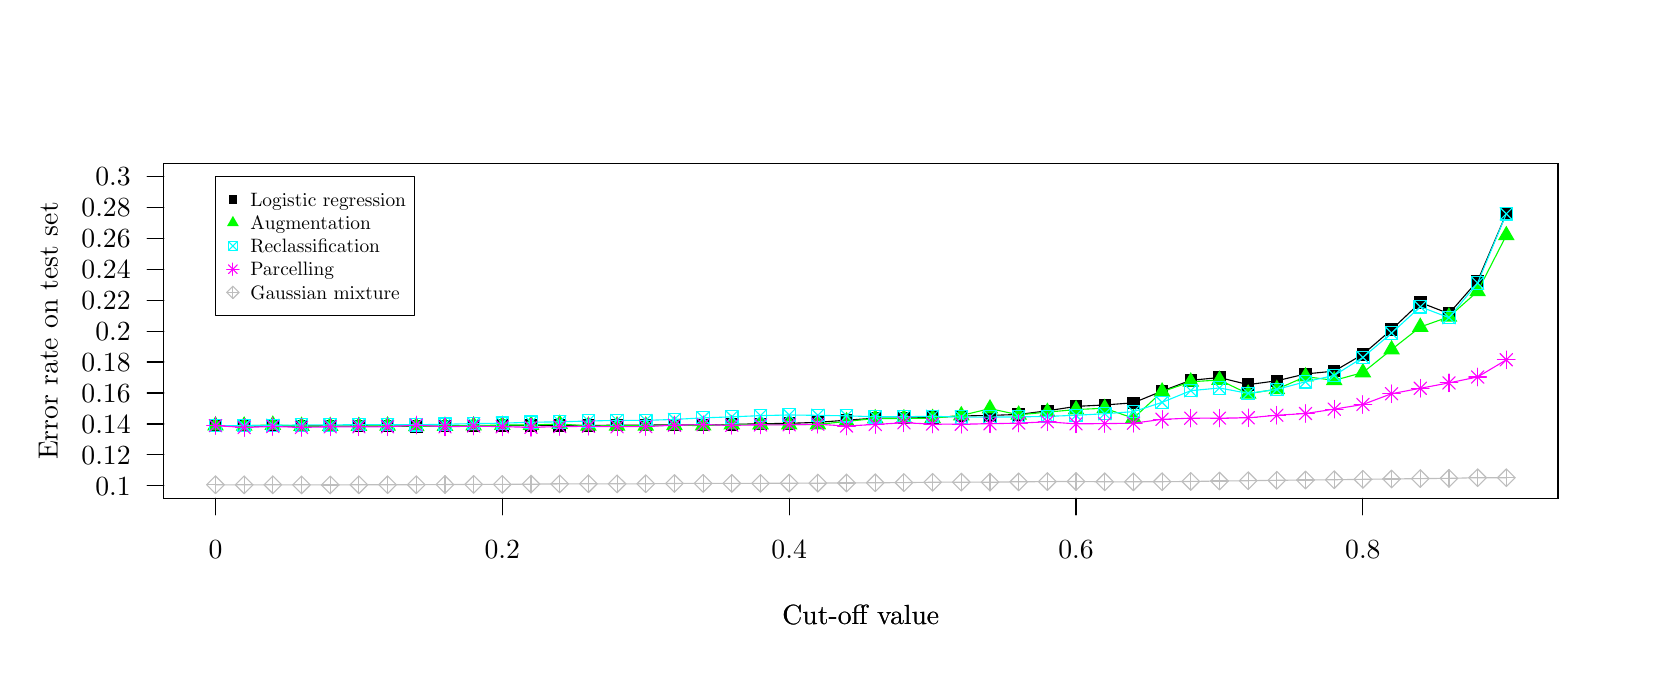
\begin{tikzpicture}[x=1pt,y=1pt]
\definecolor{fillColor}{RGB}{255,255,255}
\path[use as bounding box,fill=fillColor,fill opacity=0.00] (0,0) rectangle (578.16,231.26);
\begin{scope}
\path[clip] ( 49.20, 61.20) rectangle (552.96,182.06);
\definecolor{drawColor}{RGB}{0,0,0}

\path[draw=drawColor,line width= 0.4pt,line join=round,line cap=round] ( 67.86, 87.46) --
	( 78.22, 87.36) --
	( 88.59, 87.31) --
	( 98.95, 87.34) --
	(109.32, 87.29) --
	(119.68, 87.31) --
	(130.05, 87.29) --
	(140.42, 87.21) --
	(150.78, 87.31) --
	(161.15, 87.36) --
	(171.51, 87.47) --
	(181.88, 87.54) --
	(192.24, 87.54) --
	(202.61, 87.50) --
	(212.97, 87.62) --
	(223.34, 87.63) --
	(233.70, 87.75) --
	(244.07, 87.66) --
	(254.44, 87.89) --
	(264.80, 88.14) --
	(275.17, 88.28) --
	(285.53, 88.65) --
	(295.90, 89.42) --
	(306.26, 90.16) --
	(316.63, 90.18) --
	(326.99, 90.40) --
	(337.36, 90.94) --
	(347.72, 91.14) --
	(358.09, 91.50) --
	(368.46, 92.82) --
	(378.82, 94.41) --
	(389.19, 94.93) --
	(399.55, 95.70) --
	(409.92, 99.95) --
	(420.28,103.84) --
	(430.65,104.83) --
	(441.01,102.27) --
	(451.38,103.66) --
	(461.74,106.13) --
	(472.11,107.15) --
	(482.48,113.22) --
	(492.84,122.14) --
	(503.21,131.95) --
	(513.57,127.94) --
	(523.94,139.76) --
	(534.30,164.08);
\definecolor{fillColor}{RGB}{0,0,0}

\path[fill=fillColor] ( 65.61, 85.21) --
	( 70.11, 85.21) --
	( 70.11, 89.71) --
	( 65.61, 89.71) --
	cycle;

\path[fill=fillColor] ( 75.97, 85.11) --
	( 80.47, 85.11) --
	( 80.47, 89.61) --
	( 75.97, 89.61) --
	cycle;

\path[fill=fillColor] ( 86.34, 85.06) --
	( 90.84, 85.06) --
	( 90.84, 89.56) --
	( 86.34, 89.56) --
	cycle;

\path[fill=fillColor] ( 96.70, 85.09) --
	(101.20, 85.09) --
	(101.20, 89.59) --
	( 96.70, 89.59) --
	cycle;

\path[fill=fillColor] (107.07, 85.04) --
	(111.57, 85.04) --
	(111.57, 89.54) --
	(107.07, 89.54) --
	cycle;

\path[fill=fillColor] (117.43, 85.06) --
	(121.93, 85.06) --
	(121.93, 89.56) --
	(117.43, 89.56) --
	cycle;

\path[fill=fillColor] (127.80, 85.04) --
	(132.30, 85.04) --
	(132.30, 89.54) --
	(127.80, 89.54) --
	cycle;

\path[fill=fillColor] (138.17, 84.96) --
	(142.67, 84.96) --
	(142.67, 89.46) --
	(138.17, 89.46) --
	cycle;

\path[fill=fillColor] (148.53, 85.06) --
	(153.03, 85.06) --
	(153.03, 89.56) --
	(148.53, 89.56) --
	cycle;

\path[fill=fillColor] (158.90, 85.11) --
	(163.40, 85.11) --
	(163.40, 89.61) --
	(158.90, 89.61) --
	cycle;

\path[fill=fillColor] (169.26, 85.22) --
	(173.76, 85.22) --
	(173.76, 89.72) --
	(169.26, 89.72) --
	cycle;

\path[fill=fillColor] (179.63, 85.29) --
	(184.13, 85.29) --
	(184.13, 89.79) --
	(179.63, 89.79) --
	cycle;

\path[fill=fillColor] (189.99, 85.29) --
	(194.49, 85.29) --
	(194.49, 89.79) --
	(189.99, 89.79) --
	cycle;

\path[fill=fillColor] (200.36, 85.25) --
	(204.86, 85.25) --
	(204.86, 89.75) --
	(200.36, 89.75) --
	cycle;

\path[fill=fillColor] (210.72, 85.37) --
	(215.22, 85.37) --
	(215.22, 89.87) --
	(210.72, 89.87) --
	cycle;

\path[fill=fillColor] (221.09, 85.38) --
	(225.59, 85.38) --
	(225.59, 89.88) --
	(221.09, 89.88) --
	cycle;

\path[fill=fillColor] (231.45, 85.50) --
	(235.95, 85.50) --
	(235.95, 90.00) --
	(231.45, 90.00) --
	cycle;

\path[fill=fillColor] (241.82, 85.41) --
	(246.32, 85.41) --
	(246.32, 89.91) --
	(241.82, 89.91) --
	cycle;

\path[fill=fillColor] (252.19, 85.64) --
	(256.69, 85.64) --
	(256.69, 90.14) --
	(252.19, 90.14) --
	cycle;

\path[fill=fillColor] (262.55, 85.89) --
	(267.05, 85.89) --
	(267.05, 90.39) --
	(262.55, 90.39) --
	cycle;

\path[fill=fillColor] (272.92, 86.03) --
	(277.42, 86.03) --
	(277.42, 90.53) --
	(272.92, 90.53) --
	cycle;

\path[fill=fillColor] (283.28, 86.40) --
	(287.78, 86.40) --
	(287.78, 90.90) --
	(283.28, 90.90) --
	cycle;

\path[fill=fillColor] (293.65, 87.17) --
	(298.15, 87.17) --
	(298.15, 91.67) --
	(293.65, 91.67) --
	cycle;

\path[fill=fillColor] (304.01, 87.91) --
	(308.51, 87.91) --
	(308.51, 92.41) --
	(304.01, 92.41) --
	cycle;

\path[fill=fillColor] (314.38, 87.93) --
	(318.88, 87.93) --
	(318.88, 92.43) --
	(314.38, 92.43) --
	cycle;

\path[fill=fillColor] (324.74, 88.15) --
	(329.24, 88.15) --
	(329.24, 92.65) --
	(324.74, 92.65) --
	cycle;

\path[fill=fillColor] (335.11, 88.69) --
	(339.61, 88.69) --
	(339.61, 93.19) --
	(335.11, 93.19) --
	cycle;

\path[fill=fillColor] (345.47, 88.89) --
	(349.97, 88.89) --
	(349.97, 93.39) --
	(345.47, 93.39) --
	cycle;

\path[fill=fillColor] (355.84, 89.25) --
	(360.34, 89.25) --
	(360.34, 93.75) --
	(355.84, 93.75) --
	cycle;

\path[fill=fillColor] (366.21, 90.57) --
	(370.71, 90.57) --
	(370.71, 95.07) --
	(366.21, 95.07) --
	cycle;

\path[fill=fillColor] (376.57, 92.16) --
	(381.07, 92.16) --
	(381.07, 96.66) --
	(376.57, 96.66) --
	cycle;

\path[fill=fillColor] (386.94, 92.68) --
	(391.44, 92.68) --
	(391.44, 97.18) --
	(386.94, 97.18) --
	cycle;

\path[fill=fillColor] (397.30, 93.45) --
	(401.80, 93.45) --
	(401.80, 97.95) --
	(397.30, 97.95) --
	cycle;

\path[fill=fillColor] (407.67, 97.70) --
	(412.17, 97.70) --
	(412.17,102.20) --
	(407.67,102.20) --
	cycle;

\path[fill=fillColor] (418.03,101.59) --
	(422.53,101.59) --
	(422.53,106.09) --
	(418.03,106.09) --
	cycle;

\path[fill=fillColor] (428.40,102.58) --
	(432.90,102.58) --
	(432.90,107.08) --
	(428.40,107.08) --
	cycle;

\path[fill=fillColor] (438.76,100.02) --
	(443.26,100.02) --
	(443.26,104.52) --
	(438.76,104.52) --
	cycle;

\path[fill=fillColor] (449.13,101.41) --
	(453.63,101.41) --
	(453.63,105.91) --
	(449.13,105.91) --
	cycle;

\path[fill=fillColor] (459.49,103.88) --
	(463.99,103.88) --
	(463.99,108.38) --
	(459.49,108.38) --
	cycle;

\path[fill=fillColor] (469.86,104.90) --
	(474.36,104.90) --
	(474.36,109.40) --
	(469.86,109.40) --
	cycle;

\path[fill=fillColor] (480.23,110.97) --
	(484.73,110.97) --
	(484.73,115.47) --
	(480.23,115.47) --
	cycle;

\path[fill=fillColor] (490.59,119.89) --
	(495.09,119.89) --
	(495.09,124.39) --
	(490.59,124.39) --
	cycle;

\path[fill=fillColor] (500.96,129.70) --
	(505.46,129.70) --
	(505.46,134.20) --
	(500.96,134.20) --
	cycle;

\path[fill=fillColor] (511.32,125.69) --
	(515.82,125.69) --
	(515.82,130.19) --
	(511.32,130.19) --
	cycle;

\path[fill=fillColor] (521.69,137.51) --
	(526.19,137.51) --
	(526.19,142.01) --
	(521.69,142.01) --
	cycle;

\path[fill=fillColor] (532.05,161.83) --
	(536.55,161.83) --
	(536.55,166.33) --
	(532.05,166.33) --
	cycle;
\end{scope}
\begin{scope}
\path[clip] (  0.00,  0.00) rectangle (578.16,231.26);
\definecolor{drawColor}{RGB}{0,0,0}

\path[draw=drawColor,line width= 0.4pt,line join=round,line cap=round] ( 49.20, 61.20) --
	(552.96, 61.20) --
	(552.96,182.06) --
	( 49.20,182.06) --
	( 49.20, 61.20);
\end{scope}
\begin{scope}
\path[clip] (  0.00,  0.00) rectangle (578.16,231.26);
\definecolor{drawColor}{RGB}{0,0,0}

\node[text=drawColor,anchor=base,inner sep=0pt, outer sep=0pt, scale=  1.00] at (301.08, 15.60) {Cut-off value};

\node[text=drawColor,rotate= 90.00,anchor=base,inner sep=0pt, outer sep=0pt, scale=  1.00] at ( 10.80,121.63) {Error rate on test set};
\end{scope}
\begin{scope}
\path[clip] ( 49.20, 61.20) rectangle (552.96,182.06);
\definecolor{drawColor}{RGB}{0,255,0}

\path[draw=drawColor,line width= 0.4pt,line join=round,line cap=round] ( 67.86, 87.46) --
	( 78.22, 87.40) --
	( 88.59, 87.71) --
	( 98.95, 87.30) --
	(109.32, 87.27) --
	(119.68, 87.30) --
	(130.05, 87.43) --
	(140.42, 87.19) --
	(150.78, 87.33) --
	(161.15, 87.46) --
	(171.51, 87.66) --
	(181.88, 87.68) --
	(192.24, 88.04) --
	(202.61, 87.36) --
	(212.97, 87.44) --
	(223.34, 87.40) --
	(233.70, 87.61) --
	(244.07, 87.47) --
	(254.44, 87.86) --
	(264.80, 87.88) --
	(275.17, 87.81) --
	(285.53, 87.88) --
	(295.90, 88.98) --
	(306.26, 90.05) --
	(316.63, 90.05) --
	(326.99, 90.15) --
	(337.36, 91.14) --
	(347.72, 93.59) --
	(358.09, 91.37) --
	(368.46, 92.33) --
	(378.82, 93.27) --
	(389.19, 93.74) --
	(399.55, 90.13) --
	(409.92, 99.71) --
	(420.28,103.31) --
	(430.65,103.94) --
	(441.01, 98.98) --
	(451.38,100.63) --
	(461.74,105.16) --
	(472.11,103.82) --
	(482.48,106.63) --
	(492.84,114.95) --
	(503.21,123.09) --
	(513.57,126.77) --
	(523.94,135.96) --
	(534.30,156.20);
\definecolor{fillColor}{RGB}{0,255,0}

\path[fill=fillColor] ( 67.86, 90.96) --
	( 70.89, 85.71) --
	( 64.83, 85.71) --
	cycle;

\path[fill=fillColor] ( 78.22, 90.90) --
	( 81.25, 85.65) --
	( 75.19, 85.65) --
	cycle;

\path[fill=fillColor] ( 88.59, 91.21) --
	( 91.62, 85.96) --
	( 85.56, 85.96) --
	cycle;

\path[fill=fillColor] ( 98.95, 90.80) --
	(101.98, 85.55) --
	( 95.92, 85.55) --
	cycle;

\path[fill=fillColor] (109.32, 90.77) --
	(112.35, 85.52) --
	(106.29, 85.52) --
	cycle;

\path[fill=fillColor] (119.68, 90.80) --
	(122.72, 85.55) --
	(116.65, 85.55) --
	cycle;

\path[fill=fillColor] (130.05, 90.93) --
	(133.08, 85.68) --
	(127.02, 85.68) --
	cycle;

\path[fill=fillColor] (140.42, 90.68) --
	(143.45, 85.44) --
	(137.39, 85.44) --
	cycle;

\path[fill=fillColor] (150.78, 90.83) --
	(153.81, 85.58) --
	(147.75, 85.58) --
	cycle;

\path[fill=fillColor] (161.15, 90.96) --
	(164.18, 85.71) --
	(158.12, 85.71) --
	cycle;

\path[fill=fillColor] (171.51, 91.15) --
	(174.54, 85.91) --
	(168.48, 85.91) --
	cycle;

\path[fill=fillColor] (181.88, 91.18) --
	(184.91, 85.93) --
	(178.85, 85.93) --
	cycle;

\path[fill=fillColor] (192.24, 91.54) --
	(195.27, 86.29) --
	(189.21, 86.29) --
	cycle;

\path[fill=fillColor] (202.61, 90.86) --
	(205.64, 85.61) --
	(199.58, 85.61) --
	cycle;

\path[fill=fillColor] (212.97, 90.94) --
	(216.00, 85.69) --
	(209.94, 85.69) --
	cycle;

\path[fill=fillColor] (223.34, 90.90) --
	(226.37, 85.65) --
	(220.31, 85.65) --
	cycle;

\path[fill=fillColor] (233.70, 91.11) --
	(236.73, 85.86) --
	(230.67, 85.86) --
	cycle;

\path[fill=fillColor] (244.07, 90.97) --
	(247.10, 85.72) --
	(241.04, 85.72) --
	cycle;

\path[fill=fillColor] (254.44, 91.36) --
	(257.47, 86.11) --
	(251.41, 86.11) --
	cycle;

\path[fill=fillColor] (264.80, 91.38) --
	(267.83, 86.13) --
	(261.77, 86.13) --
	cycle;

\path[fill=fillColor] (275.17, 91.31) --
	(278.20, 86.06) --
	(272.14, 86.06) --
	cycle;

\path[fill=fillColor] (285.53, 91.38) --
	(288.56, 86.13) --
	(282.50, 86.13) --
	cycle;

\path[fill=fillColor] (295.90, 92.48) --
	(298.93, 87.23) --
	(292.87, 87.23) --
	cycle;

\path[fill=fillColor] (306.26, 93.54) --
	(309.29, 88.30) --
	(303.23, 88.30) --
	cycle;

\path[fill=fillColor] (316.63, 93.54) --
	(319.66, 88.30) --
	(313.60, 88.30) --
	cycle;

\path[fill=fillColor] (326.99, 93.64) --
	(330.02, 88.40) --
	(323.96, 88.40) --
	cycle;

\path[fill=fillColor] (337.36, 94.64) --
	(340.39, 89.39) --
	(334.33, 89.39) --
	cycle;

\path[fill=fillColor] (347.72, 97.09) --
	(350.75, 91.84) --
	(344.69, 91.84) --
	cycle;

\path[fill=fillColor] (358.09, 94.87) --
	(361.12, 89.62) --
	(355.06, 89.62) --
	cycle;

\path[fill=fillColor] (368.46, 95.83) --
	(371.49, 90.58) --
	(365.43, 90.58) --
	cycle;

\path[fill=fillColor] (378.82, 96.77) --
	(381.85, 91.52) --
	(375.79, 91.52) --
	cycle;

\path[fill=fillColor] (389.19, 97.24) --
	(392.22, 91.99) --
	(386.16, 91.99) --
	cycle;

\path[fill=fillColor] (399.55, 93.63) --
	(402.58, 88.39) --
	(396.52, 88.39) --
	cycle;

\path[fill=fillColor] (409.92,103.21) --
	(412.95, 97.96) --
	(406.89, 97.96) --
	cycle;

\path[fill=fillColor] (420.28,106.81) --
	(423.31,101.56) --
	(417.25,101.56) --
	cycle;

\path[fill=fillColor] (430.65,107.44) --
	(433.68,102.19) --
	(427.62,102.19) --
	cycle;

\path[fill=fillColor] (441.01,102.47) --
	(444.04, 97.23) --
	(437.98, 97.23) --
	cycle;

\path[fill=fillColor] (451.38,104.13) --
	(454.41, 98.88) --
	(448.35, 98.88) --
	cycle;

\path[fill=fillColor] (461.74,108.66) --
	(464.77,103.41) --
	(458.71,103.41) --
	cycle;

\path[fill=fillColor] (472.11,107.31) --
	(475.14,102.07) --
	(469.08,102.07) --
	cycle;

\path[fill=fillColor] (482.48,110.13) --
	(485.51,104.88) --
	(479.44,104.88) --
	cycle;

\path[fill=fillColor] (492.84,118.44) --
	(495.87,113.20) --
	(489.81,113.20) --
	cycle;

\path[fill=fillColor] (503.21,126.59) --
	(506.24,121.34) --
	(500.18,121.34) --
	cycle;

\path[fill=fillColor] (513.57,130.27) --
	(516.60,125.02) --
	(510.54,125.02) --
	cycle;

\path[fill=fillColor] (523.94,139.46) --
	(526.97,134.21) --
	(520.91,134.21) --
	cycle;

\path[fill=fillColor] (534.30,159.69) --
	(537.33,154.45) --
	(531.27,154.45) --
	cycle;
\end{scope}
\begin{scope}
\path[clip] (  0.00,  0.00) rectangle (578.16,231.26);
\definecolor{drawColor}{RGB}{0,0,0}

\path[draw=drawColor,line width= 0.4pt,line join=round,line cap=round] ( 49.20, 61.20) --
	(552.96, 61.20) --
	(552.96,182.06) --
	( 49.20,182.06) --
	( 49.20, 61.20);
\end{scope}
\begin{scope}
\path[clip] (  0.00,  0.00) rectangle (578.16,231.26);
\definecolor{drawColor}{RGB}{0,0,0}

%\node[text=drawColor,anchor=base,inner sep=0pt, outer sep=0pt, scale=  1.00] at (301.08, 15.60) {Cut-off value};

%\node[text=drawColor,rotate= 90.00,anchor=base,inner sep=0pt, outer sep=0pt, scale=  1.00] at ( 10.80,121.63) {Error rate on test set};
\end{scope}
\begin{scope}
\path[clip] ( 49.20, 61.20) rectangle (552.96,182.06);
\definecolor{drawColor}{RGB}{0,255,255}

\path[draw=drawColor,line width= 0.4pt,line join=round,line cap=round] ( 67.86, 87.46) --
	( 78.22, 87.46) --
	( 88.59, 87.57) --
	( 98.95, 87.71) --
	(109.32, 87.72) --
	(119.68, 87.80) --
	(130.05, 87.80) --
	(140.42, 87.77) --
	(150.78, 87.95) --
	(161.15, 88.18) --
	(171.51, 88.34) --
	(181.88, 88.68) --
	(192.24, 88.83) --
	(202.61, 89.13) --
	(212.97, 89.35) --
	(223.34, 89.35) --
	(233.70, 89.70) --
	(244.07, 90.26) --
	(254.44, 90.63) --
	(264.80, 91.07) --
	(275.17, 91.31) --
	(285.53, 91.17) --
	(295.90, 91.00) --
	(306.26, 90.67) --
	(316.63, 90.68) --
	(326.99, 90.83) --
	(337.36, 90.55) --
	(347.72, 90.55) --
	(358.09, 90.60) --
	(368.46, 90.80) --
	(378.82, 91.19) --
	(389.19, 91.77) --
	(399.55, 92.50) --
	(409.92, 95.86) --
	(420.28,100.09) --
	(430.65,101.06) --
	(441.01, 99.12) --
	(451.38,100.54) --
	(461.74,103.32) --
	(472.11,105.58) --
	(482.48,112.11) --
	(492.84,120.89) --
	(503.21,130.41) --
	(513.57,126.47) --
	(523.94,139.00) --
	(534.30,164.00);

\path[draw=drawColor,line width= 0.4pt,line join=round,line cap=round] ( 65.61, 85.21) rectangle ( 70.11, 89.71);

\path[draw=drawColor,line width= 0.4pt,line join=round,line cap=round] ( 65.61, 85.21) -- ( 70.11, 89.71);

\path[draw=drawColor,line width= 0.4pt,line join=round,line cap=round] ( 65.61, 89.71) -- ( 70.11, 85.21);

\path[draw=drawColor,line width= 0.4pt,line join=round,line cap=round] ( 75.97, 85.21) rectangle ( 80.47, 89.71);

\path[draw=drawColor,line width= 0.4pt,line join=round,line cap=round] ( 75.97, 85.21) -- ( 80.47, 89.71);

\path[draw=drawColor,line width= 0.4pt,line join=round,line cap=round] ( 75.97, 89.71) -- ( 80.47, 85.21);

\path[draw=drawColor,line width= 0.4pt,line join=round,line cap=round] ( 86.34, 85.32) rectangle ( 90.84, 89.82);

\path[draw=drawColor,line width= 0.4pt,line join=round,line cap=round] ( 86.34, 85.32) -- ( 90.84, 89.82);

\path[draw=drawColor,line width= 0.4pt,line join=round,line cap=round] ( 86.34, 89.82) -- ( 90.84, 85.32);

\path[draw=drawColor,line width= 0.4pt,line join=round,line cap=round] ( 96.70, 85.46) rectangle (101.20, 89.96);

\path[draw=drawColor,line width= 0.4pt,line join=round,line cap=round] ( 96.70, 85.46) -- (101.20, 89.96);

\path[draw=drawColor,line width= 0.4pt,line join=round,line cap=round] ( 96.70, 89.96) -- (101.20, 85.46);

\path[draw=drawColor,line width= 0.4pt,line join=round,line cap=round] (107.07, 85.47) rectangle (111.57, 89.97);

\path[draw=drawColor,line width= 0.4pt,line join=round,line cap=round] (107.07, 85.47) -- (111.57, 89.97);

\path[draw=drawColor,line width= 0.4pt,line join=round,line cap=round] (107.07, 89.97) -- (111.57, 85.47);

\path[draw=drawColor,line width= 0.4pt,line join=round,line cap=round] (117.43, 85.55) rectangle (121.93, 90.05);

\path[draw=drawColor,line width= 0.4pt,line join=round,line cap=round] (117.43, 85.55) -- (121.93, 90.05);

\path[draw=drawColor,line width= 0.4pt,line join=round,line cap=round] (117.43, 90.05) -- (121.93, 85.55);

\path[draw=drawColor,line width= 0.4pt,line join=round,line cap=round] (127.80, 85.55) rectangle (132.30, 90.05);

\path[draw=drawColor,line width= 0.4pt,line join=round,line cap=round] (127.80, 85.55) -- (132.30, 90.05);

\path[draw=drawColor,line width= 0.4pt,line join=round,line cap=round] (127.80, 90.05) -- (132.30, 85.55);

\path[draw=drawColor,line width= 0.4pt,line join=round,line cap=round] (138.17, 85.52) rectangle (142.67, 90.02);

\path[draw=drawColor,line width= 0.4pt,line join=round,line cap=round] (138.17, 85.52) -- (142.67, 90.02);

\path[draw=drawColor,line width= 0.4pt,line join=round,line cap=round] (138.17, 90.02) -- (142.67, 85.52);

\path[draw=drawColor,line width= 0.4pt,line join=round,line cap=round] (148.53, 85.70) rectangle (153.03, 90.20);

\path[draw=drawColor,line width= 0.4pt,line join=round,line cap=round] (148.53, 85.70) -- (153.03, 90.20);

\path[draw=drawColor,line width= 0.4pt,line join=round,line cap=round] (148.53, 90.20) -- (153.03, 85.70);

\path[draw=drawColor,line width= 0.4pt,line join=round,line cap=round] (158.90, 85.93) rectangle (163.40, 90.43);

\path[draw=drawColor,line width= 0.4pt,line join=round,line cap=round] (158.90, 85.93) -- (163.40, 90.43);

\path[draw=drawColor,line width= 0.4pt,line join=round,line cap=round] (158.90, 90.43) -- (163.40, 85.93);

\path[draw=drawColor,line width= 0.4pt,line join=round,line cap=round] (169.26, 86.09) rectangle (173.76, 90.59);

\path[draw=drawColor,line width= 0.4pt,line join=round,line cap=round] (169.26, 86.09) -- (173.76, 90.59);

\path[draw=drawColor,line width= 0.4pt,line join=round,line cap=round] (169.26, 90.59) -- (173.76, 86.09);

\path[draw=drawColor,line width= 0.4pt,line join=round,line cap=round] (179.63, 86.43) rectangle (184.13, 90.93);

\path[draw=drawColor,line width= 0.4pt,line join=round,line cap=round] (179.63, 86.43) -- (184.13, 90.93);

\path[draw=drawColor,line width= 0.4pt,line join=round,line cap=round] (179.63, 90.93) -- (184.13, 86.43);

\path[draw=drawColor,line width= 0.4pt,line join=round,line cap=round] (189.99, 86.58) rectangle (194.49, 91.08);

\path[draw=drawColor,line width= 0.4pt,line join=round,line cap=round] (189.99, 86.58) -- (194.49, 91.08);

\path[draw=drawColor,line width= 0.4pt,line join=round,line cap=round] (189.99, 91.08) -- (194.49, 86.58);

\path[draw=drawColor,line width= 0.4pt,line join=round,line cap=round] (200.36, 86.88) rectangle (204.86, 91.38);

\path[draw=drawColor,line width= 0.4pt,line join=round,line cap=round] (200.36, 86.88) -- (204.86, 91.38);

\path[draw=drawColor,line width= 0.4pt,line join=round,line cap=round] (200.36, 91.38) -- (204.86, 86.88);

\path[draw=drawColor,line width= 0.4pt,line join=round,line cap=round] (210.72, 87.10) rectangle (215.22, 91.60);

\path[draw=drawColor,line width= 0.4pt,line join=round,line cap=round] (210.72, 87.10) -- (215.22, 91.60);

\path[draw=drawColor,line width= 0.4pt,line join=round,line cap=round] (210.72, 91.60) -- (215.22, 87.10);

\path[draw=drawColor,line width= 0.4pt,line join=round,line cap=round] (221.09, 87.10) rectangle (225.59, 91.60);

\path[draw=drawColor,line width= 0.4pt,line join=round,line cap=round] (221.09, 87.10) -- (225.59, 91.60);

\path[draw=drawColor,line width= 0.4pt,line join=round,line cap=round] (221.09, 91.60) -- (225.59, 87.10);

\path[draw=drawColor,line width= 0.4pt,line join=round,line cap=round] (231.45, 87.45) rectangle (235.95, 91.95);

\path[draw=drawColor,line width= 0.4pt,line join=round,line cap=round] (231.45, 87.45) -- (235.95, 91.95);

\path[draw=drawColor,line width= 0.4pt,line join=round,line cap=round] (231.45, 91.95) -- (235.95, 87.45);

\path[draw=drawColor,line width= 0.4pt,line join=round,line cap=round] (241.82, 88.01) rectangle (246.32, 92.51);

\path[draw=drawColor,line width= 0.4pt,line join=round,line cap=round] (241.82, 88.01) -- (246.32, 92.51);

\path[draw=drawColor,line width= 0.4pt,line join=round,line cap=round] (241.82, 92.51) -- (246.32, 88.01);

\path[draw=drawColor,line width= 0.4pt,line join=round,line cap=round] (252.19, 88.38) rectangle (256.69, 92.88);

\path[draw=drawColor,line width= 0.4pt,line join=round,line cap=round] (252.19, 88.38) -- (256.69, 92.88);

\path[draw=drawColor,line width= 0.4pt,line join=round,line cap=round] (252.19, 92.88) -- (256.69, 88.38);

\path[draw=drawColor,line width= 0.4pt,line join=round,line cap=round] (262.55, 88.82) rectangle (267.05, 93.32);

\path[draw=drawColor,line width= 0.4pt,line join=round,line cap=round] (262.55, 88.82) -- (267.05, 93.32);

\path[draw=drawColor,line width= 0.4pt,line join=round,line cap=round] (262.55, 93.32) -- (267.05, 88.82);

\path[draw=drawColor,line width= 0.4pt,line join=round,line cap=round] (272.92, 89.06) rectangle (277.42, 93.56);

\path[draw=drawColor,line width= 0.4pt,line join=round,line cap=round] (272.92, 89.06) -- (277.42, 93.56);

\path[draw=drawColor,line width= 0.4pt,line join=round,line cap=round] (272.92, 93.56) -- (277.42, 89.06);

\path[draw=drawColor,line width= 0.4pt,line join=round,line cap=round] (283.28, 88.92) rectangle (287.78, 93.42);

\path[draw=drawColor,line width= 0.4pt,line join=round,line cap=round] (283.28, 88.92) -- (287.78, 93.42);

\path[draw=drawColor,line width= 0.4pt,line join=round,line cap=round] (283.28, 93.42) -- (287.78, 88.92);

\path[draw=drawColor,line width= 0.4pt,line join=round,line cap=round] (293.65, 88.75) rectangle (298.15, 93.25);

\path[draw=drawColor,line width= 0.4pt,line join=round,line cap=round] (293.65, 88.75) -- (298.15, 93.25);

\path[draw=drawColor,line width= 0.4pt,line join=round,line cap=round] (293.65, 93.25) -- (298.15, 88.75);

\path[draw=drawColor,line width= 0.4pt,line join=round,line cap=round] (304.01, 88.42) rectangle (308.51, 92.92);

\path[draw=drawColor,line width= 0.4pt,line join=round,line cap=round] (304.01, 88.42) -- (308.51, 92.92);

\path[draw=drawColor,line width= 0.4pt,line join=round,line cap=round] (304.01, 92.92) -- (308.51, 88.42);

\path[draw=drawColor,line width= 0.4pt,line join=round,line cap=round] (314.38, 88.43) rectangle (318.88, 92.93);

\path[draw=drawColor,line width= 0.4pt,line join=round,line cap=round] (314.38, 88.43) -- (318.88, 92.93);

\path[draw=drawColor,line width= 0.4pt,line join=round,line cap=round] (314.38, 92.93) -- (318.88, 88.43);

\path[draw=drawColor,line width= 0.4pt,line join=round,line cap=round] (324.74, 88.58) rectangle (329.24, 93.08);

\path[draw=drawColor,line width= 0.4pt,line join=round,line cap=round] (324.74, 88.58) -- (329.24, 93.08);

\path[draw=drawColor,line width= 0.4pt,line join=round,line cap=round] (324.74, 93.08) -- (329.24, 88.58);

\path[draw=drawColor,line width= 0.4pt,line join=round,line cap=round] (335.11, 88.30) rectangle (339.61, 92.80);

\path[draw=drawColor,line width= 0.4pt,line join=round,line cap=round] (335.11, 88.30) -- (339.61, 92.80);

\path[draw=drawColor,line width= 0.4pt,line join=round,line cap=round] (335.11, 92.80) -- (339.61, 88.30);

\path[draw=drawColor,line width= 0.4pt,line join=round,line cap=round] (345.47, 88.30) rectangle (349.97, 92.80);

\path[draw=drawColor,line width= 0.4pt,line join=round,line cap=round] (345.47, 88.30) -- (349.97, 92.80);

\path[draw=drawColor,line width= 0.4pt,line join=round,line cap=round] (345.47, 92.80) -- (349.97, 88.30);

\path[draw=drawColor,line width= 0.4pt,line join=round,line cap=round] (355.84, 88.35) rectangle (360.34, 92.85);

\path[draw=drawColor,line width= 0.4pt,line join=round,line cap=round] (355.84, 88.35) -- (360.34, 92.85);

\path[draw=drawColor,line width= 0.4pt,line join=round,line cap=round] (355.84, 92.85) -- (360.34, 88.35);

\path[draw=drawColor,line width= 0.4pt,line join=round,line cap=round] (366.21, 88.55) rectangle (370.71, 93.05);

\path[draw=drawColor,line width= 0.4pt,line join=round,line cap=round] (366.21, 88.55) -- (370.71, 93.05);

\path[draw=drawColor,line width= 0.4pt,line join=round,line cap=round] (366.21, 93.05) -- (370.71, 88.55);

\path[draw=drawColor,line width= 0.4pt,line join=round,line cap=round] (376.57, 88.94) rectangle (381.07, 93.44);

\path[draw=drawColor,line width= 0.4pt,line join=round,line cap=round] (376.57, 88.94) -- (381.07, 93.44);

\path[draw=drawColor,line width= 0.4pt,line join=round,line cap=round] (376.57, 93.44) -- (381.07, 88.94);

\path[draw=drawColor,line width= 0.4pt,line join=round,line cap=round] (386.94, 89.52) rectangle (391.44, 94.02);

\path[draw=drawColor,line width= 0.4pt,line join=round,line cap=round] (386.94, 89.52) -- (391.44, 94.02);

\path[draw=drawColor,line width= 0.4pt,line join=round,line cap=round] (386.94, 94.02) -- (391.44, 89.52);

\path[draw=drawColor,line width= 0.4pt,line join=round,line cap=round] (397.30, 90.25) rectangle (401.80, 94.75);

\path[draw=drawColor,line width= 0.4pt,line join=round,line cap=round] (397.30, 90.25) -- (401.80, 94.75);

\path[draw=drawColor,line width= 0.4pt,line join=round,line cap=round] (397.30, 94.75) -- (401.80, 90.25);

\path[draw=drawColor,line width= 0.4pt,line join=round,line cap=round] (407.67, 93.61) rectangle (412.17, 98.11);

\path[draw=drawColor,line width= 0.4pt,line join=round,line cap=round] (407.67, 93.61) -- (412.17, 98.11);

\path[draw=drawColor,line width= 0.4pt,line join=round,line cap=round] (407.67, 98.11) -- (412.17, 93.61);

\path[draw=drawColor,line width= 0.4pt,line join=round,line cap=round] (418.03, 97.84) rectangle (422.53,102.34);

\path[draw=drawColor,line width= 0.4pt,line join=round,line cap=round] (418.03, 97.84) -- (422.53,102.34);

\path[draw=drawColor,line width= 0.4pt,line join=round,line cap=round] (418.03,102.34) -- (422.53, 97.84);

\path[draw=drawColor,line width= 0.4pt,line join=round,line cap=round] (428.40, 98.81) rectangle (432.90,103.31);

\path[draw=drawColor,line width= 0.4pt,line join=round,line cap=round] (428.40, 98.81) -- (432.90,103.31);

\path[draw=drawColor,line width= 0.4pt,line join=round,line cap=round] (428.40,103.31) -- (432.90, 98.81);

\path[draw=drawColor,line width= 0.4pt,line join=round,line cap=round] (438.76, 96.87) rectangle (443.26,101.37);

\path[draw=drawColor,line width= 0.4pt,line join=round,line cap=round] (438.76, 96.87) -- (443.26,101.37);

\path[draw=drawColor,line width= 0.4pt,line join=round,line cap=round] (438.76,101.37) -- (443.26, 96.87);

\path[draw=drawColor,line width= 0.4pt,line join=round,line cap=round] (449.13, 98.29) rectangle (453.63,102.79);

\path[draw=drawColor,line width= 0.4pt,line join=round,line cap=round] (449.13, 98.29) -- (453.63,102.79);

\path[draw=drawColor,line width= 0.4pt,line join=round,line cap=round] (449.13,102.79) -- (453.63, 98.29);

\path[draw=drawColor,line width= 0.4pt,line join=round,line cap=round] (459.49,101.07) rectangle (463.99,105.57);

\path[draw=drawColor,line width= 0.4pt,line join=round,line cap=round] (459.49,101.07) -- (463.99,105.57);

\path[draw=drawColor,line width= 0.4pt,line join=round,line cap=round] (459.49,105.57) -- (463.99,101.07);

\path[draw=drawColor,line width= 0.4pt,line join=round,line cap=round] (469.86,103.33) rectangle (474.36,107.83);

\path[draw=drawColor,line width= 0.4pt,line join=round,line cap=round] (469.86,103.33) -- (474.36,107.83);

\path[draw=drawColor,line width= 0.4pt,line join=round,line cap=round] (469.86,107.83) -- (474.36,103.33);

\path[draw=drawColor,line width= 0.4pt,line join=round,line cap=round] (480.23,109.86) rectangle (484.73,114.36);

\path[draw=drawColor,line width= 0.4pt,line join=round,line cap=round] (480.23,109.86) -- (484.73,114.36);

\path[draw=drawColor,line width= 0.4pt,line join=round,line cap=round] (480.23,114.36) -- (484.73,109.86);

\path[draw=drawColor,line width= 0.4pt,line join=round,line cap=round] (490.59,118.64) rectangle (495.09,123.14);

\path[draw=drawColor,line width= 0.4pt,line join=round,line cap=round] (490.59,118.64) -- (495.09,123.14);

\path[draw=drawColor,line width= 0.4pt,line join=round,line cap=round] (490.59,123.14) -- (495.09,118.64);

\path[draw=drawColor,line width= 0.4pt,line join=round,line cap=round] (500.96,128.16) rectangle (505.46,132.66);

\path[draw=drawColor,line width= 0.4pt,line join=round,line cap=round] (500.96,128.16) -- (505.46,132.66);

\path[draw=drawColor,line width= 0.4pt,line join=round,line cap=round] (500.96,132.66) -- (505.46,128.16);

\path[draw=drawColor,line width= 0.4pt,line join=round,line cap=round] (511.32,124.22) rectangle (515.82,128.72);

\path[draw=drawColor,line width= 0.4pt,line join=round,line cap=round] (511.32,124.22) -- (515.82,128.72);

\path[draw=drawColor,line width= 0.4pt,line join=round,line cap=round] (511.32,128.72) -- (515.82,124.22);

\path[draw=drawColor,line width= 0.4pt,line join=round,line cap=round] (521.69,136.75) rectangle (526.19,141.25);

\path[draw=drawColor,line width= 0.4pt,line join=round,line cap=round] (521.69,136.75) -- (526.19,141.25);

\path[draw=drawColor,line width= 0.4pt,line join=round,line cap=round] (521.69,141.25) -- (526.19,136.75);

\path[draw=drawColor,line width= 0.4pt,line join=round,line cap=round] (532.05,161.75) rectangle (536.55,166.25);

\path[draw=drawColor,line width= 0.4pt,line join=round,line cap=round] (532.05,161.75) -- (536.55,166.25);

\path[draw=drawColor,line width= 0.4pt,line join=round,line cap=round] (532.05,166.25) -- (536.55,161.75);
\end{scope}
\begin{scope}
\path[clip] (  0.00,  0.00) rectangle (578.16,231.26);
\definecolor{drawColor}{RGB}{0,0,0}

\path[draw=drawColor,line width= 0.4pt,line join=round,line cap=round] ( 49.20, 61.20) --
	(552.96, 61.20) --
	(552.96,182.06) --
	( 49.20,182.06) --
	( 49.20, 61.20);
\end{scope}
\begin{scope}
\path[clip] (  0.00,  0.00) rectangle (578.16,231.26);
\definecolor{drawColor}{RGB}{0,0,0}

%\node[text=drawColor,anchor=base,inner sep=0pt, outer sep=0pt, scale=  1.00] at (301.08, 15.60) {Cut-off value};

%\node[text=drawColor,rotate= 90.00,anchor=base,inner sep=0pt, outer sep=0pt, scale=  1.00] at ( 10.80,121.63) {Error rate on test set};
\end{scope}
\begin{scope}
\path[clip] ( 49.20, 61.20) rectangle (552.96,182.06);
\definecolor{drawColor}{RGB}{255,0,255}

\path[draw=drawColor,line width= 0.4pt,line join=round,line cap=round] ( 67.86, 87.46) --
	( 78.22, 86.80) --
	( 88.59, 87.15) --
	( 98.95, 86.82) --
	(109.32, 87.02) --
	(119.68, 87.02) --
	(130.05, 87.02) --
	(140.42, 87.66) --
	(150.78, 87.01) --
	(161.15, 87.30) --
	(171.51, 87.07) --
	(181.88, 86.86) --
	(192.24, 87.10) --
	(202.61, 87.20) --
	(212.97, 87.06) --
	(223.34, 87.11) --
	(233.70, 87.63) --
	(244.07, 87.79) --
	(254.44, 87.59) --
	(264.80, 87.72) --
	(275.17, 87.76) --
	(285.53, 87.97) --
	(295.90, 87.30) --
	(306.26, 87.89) --
	(316.63, 88.49) --
	(326.99, 88.02) --
	(337.36, 87.98) --
	(347.72, 88.13) --
	(358.09, 88.37) --
	(368.46, 88.83) --
	(378.82, 88.10) --
	(389.19, 88.19) --
	(399.55, 88.32) --
	(409.92, 89.73) --
	(420.28, 90.16) --
	(430.65, 90.17) --
	(441.01, 90.27) --
	(451.38, 91.21) --
	(461.74, 91.83) --
	(472.11, 93.41) --
	(482.48, 95.11) --
	(492.84, 98.99) --
	(503.21,100.95) --
	(513.57,102.90) --
	(523.94,105.04) --
	(534.30,111.23);

\path[draw=drawColor,line width= 0.4pt,line join=round,line cap=round] ( 65.61, 85.21) -- ( 70.11, 89.71);

\path[draw=drawColor,line width= 0.4pt,line join=round,line cap=round] ( 65.61, 89.71) -- ( 70.11, 85.21);

\path[draw=drawColor,line width= 0.4pt,line join=round,line cap=round] ( 64.68, 87.46) -- ( 71.04, 87.46);

\path[draw=drawColor,line width= 0.4pt,line join=round,line cap=round] ( 67.86, 84.28) -- ( 67.86, 90.64);

\path[draw=drawColor,line width= 0.4pt,line join=round,line cap=round] ( 75.97, 84.55) -- ( 80.47, 89.05);

\path[draw=drawColor,line width= 0.4pt,line join=round,line cap=round] ( 75.97, 89.05) -- ( 80.47, 84.55);

\path[draw=drawColor,line width= 0.4pt,line join=round,line cap=round] ( 75.04, 86.80) -- ( 81.41, 86.80);

\path[draw=drawColor,line width= 0.4pt,line join=round,line cap=round] ( 78.22, 83.62) -- ( 78.22, 89.98);

\path[draw=drawColor,line width= 0.4pt,line join=round,line cap=round] ( 86.34, 84.90) -- ( 90.84, 89.40);

\path[draw=drawColor,line width= 0.4pt,line join=round,line cap=round] ( 86.34, 89.40) -- ( 90.84, 84.90);

\path[draw=drawColor,line width= 0.4pt,line join=round,line cap=round] ( 85.41, 87.15) -- ( 91.77, 87.15);

\path[draw=drawColor,line width= 0.4pt,line join=round,line cap=round] ( 88.59, 83.96) -- ( 88.59, 90.33);

\path[draw=drawColor,line width= 0.4pt,line join=round,line cap=round] ( 96.70, 84.57) -- (101.20, 89.07);

\path[draw=drawColor,line width= 0.4pt,line join=round,line cap=round] ( 96.70, 89.07) -- (101.20, 84.57);

\path[draw=drawColor,line width= 0.4pt,line join=round,line cap=round] ( 95.77, 86.82) -- (102.14, 86.82);

\path[draw=drawColor,line width= 0.4pt,line join=round,line cap=round] ( 98.95, 83.63) -- ( 98.95, 90.00);

\path[draw=drawColor,line width= 0.4pt,line join=round,line cap=round] (107.07, 84.77) -- (111.57, 89.27);

\path[draw=drawColor,line width= 0.4pt,line join=round,line cap=round] (107.07, 89.27) -- (111.57, 84.77);

\path[draw=drawColor,line width= 0.4pt,line join=round,line cap=round] (106.14, 87.02) -- (112.50, 87.02);

\path[draw=drawColor,line width= 0.4pt,line join=round,line cap=round] (109.32, 83.84) -- (109.32, 90.20);

\path[draw=drawColor,line width= 0.4pt,line join=round,line cap=round] (117.43, 84.77) -- (121.93, 89.27);

\path[draw=drawColor,line width= 0.4pt,line join=round,line cap=round] (117.43, 89.27) -- (121.93, 84.77);

\path[draw=drawColor,line width= 0.4pt,line join=round,line cap=round] (116.50, 87.02) -- (122.87, 87.02);

\path[draw=drawColor,line width= 0.4pt,line join=round,line cap=round] (119.68, 83.84) -- (119.68, 90.20);

\path[draw=drawColor,line width= 0.4pt,line join=round,line cap=round] (127.80, 84.77) -- (132.30, 89.27);

\path[draw=drawColor,line width= 0.4pt,line join=round,line cap=round] (127.80, 89.27) -- (132.30, 84.77);

\path[draw=drawColor,line width= 0.4pt,line join=round,line cap=round] (126.87, 87.02) -- (133.23, 87.02);

\path[draw=drawColor,line width= 0.4pt,line join=round,line cap=round] (130.05, 83.84) -- (130.05, 90.21);

\path[draw=drawColor,line width= 0.4pt,line join=round,line cap=round] (138.17, 85.41) -- (142.67, 89.91);

\path[draw=drawColor,line width= 0.4pt,line join=round,line cap=round] (138.17, 89.91) -- (142.67, 85.41);

\path[draw=drawColor,line width= 0.4pt,line join=round,line cap=round] (137.23, 87.66) -- (143.60, 87.66);

\path[draw=drawColor,line width= 0.4pt,line join=round,line cap=round] (140.42, 84.48) -- (140.42, 90.84);

\path[draw=drawColor,line width= 0.4pt,line join=round,line cap=round] (148.53, 84.76) -- (153.03, 89.26);

\path[draw=drawColor,line width= 0.4pt,line join=round,line cap=round] (148.53, 89.26) -- (153.03, 84.76);

\path[draw=drawColor,line width= 0.4pt,line join=round,line cap=round] (147.60, 87.01) -- (153.96, 87.01);

\path[draw=drawColor,line width= 0.4pt,line join=round,line cap=round] (150.78, 83.83) -- (150.78, 90.19);

\path[draw=drawColor,line width= 0.4pt,line join=round,line cap=round] (158.90, 85.05) -- (163.40, 89.55);

\path[draw=drawColor,line width= 0.4pt,line join=round,line cap=round] (158.90, 89.55) -- (163.40, 85.05);

\path[draw=drawColor,line width= 0.4pt,line join=round,line cap=round] (157.96, 87.30) -- (164.33, 87.30);

\path[draw=drawColor,line width= 0.4pt,line join=round,line cap=round] (161.15, 84.12) -- (161.15, 90.49);

\path[draw=drawColor,line width= 0.4pt,line join=round,line cap=round] (169.26, 84.82) -- (173.76, 89.32);

\path[draw=drawColor,line width= 0.4pt,line join=round,line cap=round] (169.26, 89.32) -- (173.76, 84.82);

\path[draw=drawColor,line width= 0.4pt,line join=round,line cap=round] (168.33, 87.07) -- (174.69, 87.07);

\path[draw=drawColor,line width= 0.4pt,line join=round,line cap=round] (171.51, 83.89) -- (171.51, 90.26);

\path[draw=drawColor,line width= 0.4pt,line join=round,line cap=round] (179.63, 84.61) -- (184.13, 89.11);

\path[draw=drawColor,line width= 0.4pt,line join=round,line cap=round] (179.63, 89.11) -- (184.13, 84.61);

\path[draw=drawColor,line width= 0.4pt,line join=round,line cap=round] (178.70, 86.86) -- (185.06, 86.86);

\path[draw=drawColor,line width= 0.4pt,line join=round,line cap=round] (181.88, 83.67) -- (181.88, 90.04);

\path[draw=drawColor,line width= 0.4pt,line join=round,line cap=round] (189.99, 84.85) -- (194.49, 89.35);

\path[draw=drawColor,line width= 0.4pt,line join=round,line cap=round] (189.99, 89.35) -- (194.49, 84.85);

\path[draw=drawColor,line width= 0.4pt,line join=round,line cap=round] (189.06, 87.10) -- (195.42, 87.10);

\path[draw=drawColor,line width= 0.4pt,line join=round,line cap=round] (192.24, 83.91) -- (192.24, 90.28);

\path[draw=drawColor,line width= 0.4pt,line join=round,line cap=round] (200.36, 84.95) -- (204.86, 89.45);

\path[draw=drawColor,line width= 0.4pt,line join=round,line cap=round] (200.36, 89.45) -- (204.86, 84.95);

\path[draw=drawColor,line width= 0.4pt,line join=round,line cap=round] (199.43, 87.20) -- (205.79, 87.20);

\path[draw=drawColor,line width= 0.4pt,line join=round,line cap=round] (202.61, 84.01) -- (202.61, 90.38);

\path[draw=drawColor,line width= 0.4pt,line join=round,line cap=round] (210.72, 84.81) -- (215.22, 89.31);

\path[draw=drawColor,line width= 0.4pt,line join=round,line cap=round] (210.72, 89.31) -- (215.22, 84.81);

\path[draw=drawColor,line width= 0.4pt,line join=round,line cap=round] (209.79, 87.06) -- (216.16, 87.06);

\path[draw=drawColor,line width= 0.4pt,line join=round,line cap=round] (212.97, 83.88) -- (212.97, 90.24);

\path[draw=drawColor,line width= 0.4pt,line join=round,line cap=round] (221.09, 84.86) -- (225.59, 89.36);

\path[draw=drawColor,line width= 0.4pt,line join=round,line cap=round] (221.09, 89.36) -- (225.59, 84.86);

\path[draw=drawColor,line width= 0.4pt,line join=round,line cap=round] (220.16, 87.11) -- (226.52, 87.11);

\path[draw=drawColor,line width= 0.4pt,line join=round,line cap=round] (223.34, 83.93) -- (223.34, 90.29);

\path[draw=drawColor,line width= 0.4pt,line join=round,line cap=round] (231.45, 85.38) -- (235.95, 89.88);

\path[draw=drawColor,line width= 0.4pt,line join=round,line cap=round] (231.45, 89.88) -- (235.95, 85.38);

\path[draw=drawColor,line width= 0.4pt,line join=round,line cap=round] (230.52, 87.63) -- (236.89, 87.63);

\path[draw=drawColor,line width= 0.4pt,line join=round,line cap=round] (233.70, 84.45) -- (233.70, 90.81);

\path[draw=drawColor,line width= 0.4pt,line join=round,line cap=round] (241.82, 85.54) -- (246.32, 90.04);

\path[draw=drawColor,line width= 0.4pt,line join=round,line cap=round] (241.82, 90.04) -- (246.32, 85.54);

\path[draw=drawColor,line width= 0.4pt,line join=round,line cap=round] (240.89, 87.79) -- (247.25, 87.79);

\path[draw=drawColor,line width= 0.4pt,line join=round,line cap=round] (244.07, 84.61) -- (244.07, 90.97);

\path[draw=drawColor,line width= 0.4pt,line join=round,line cap=round] (252.19, 85.34) -- (256.69, 89.84);

\path[draw=drawColor,line width= 0.4pt,line join=round,line cap=round] (252.19, 89.84) -- (256.69, 85.34);

\path[draw=drawColor,line width= 0.4pt,line join=round,line cap=round] (251.25, 87.59) -- (257.62, 87.59);

\path[draw=drawColor,line width= 0.4pt,line join=round,line cap=round] (254.44, 84.41) -- (254.44, 90.77);

\path[draw=drawColor,line width= 0.4pt,line join=round,line cap=round] (262.55, 85.47) -- (267.05, 89.97);

\path[draw=drawColor,line width= 0.4pt,line join=round,line cap=round] (262.55, 89.97) -- (267.05, 85.47);

\path[draw=drawColor,line width= 0.4pt,line join=round,line cap=round] (261.62, 87.72) -- (267.98, 87.72);

\path[draw=drawColor,line width= 0.4pt,line join=round,line cap=round] (264.80, 84.54) -- (264.80, 90.90);

\path[draw=drawColor,line width= 0.4pt,line join=round,line cap=round] (272.92, 85.51) -- (277.42, 90.01);

\path[draw=drawColor,line width= 0.4pt,line join=round,line cap=round] (272.92, 90.01) -- (277.42, 85.51);

\path[draw=drawColor,line width= 0.4pt,line join=round,line cap=round] (271.98, 87.76) -- (278.35, 87.76);

\path[draw=drawColor,line width= 0.4pt,line join=round,line cap=round] (275.17, 84.58) -- (275.17, 90.94);

\path[draw=drawColor,line width= 0.4pt,line join=round,line cap=round] (283.28, 85.72) -- (287.78, 90.22);

\path[draw=drawColor,line width= 0.4pt,line join=round,line cap=round] (283.28, 90.22) -- (287.78, 85.72);

\path[draw=drawColor,line width= 0.4pt,line join=round,line cap=round] (282.35, 87.97) -- (288.71, 87.97);

\path[draw=drawColor,line width= 0.4pt,line join=round,line cap=round] (285.53, 84.79) -- (285.53, 91.16);

\path[draw=drawColor,line width= 0.4pt,line join=round,line cap=round] (293.65, 85.05) -- (298.15, 89.55);

\path[draw=drawColor,line width= 0.4pt,line join=round,line cap=round] (293.65, 89.55) -- (298.15, 85.05);

\path[draw=drawColor,line width= 0.4pt,line join=round,line cap=round] (292.72, 87.30) -- (299.08, 87.30);

\path[draw=drawColor,line width= 0.4pt,line join=round,line cap=round] (295.90, 84.12) -- (295.90, 90.49);

\path[draw=drawColor,line width= 0.4pt,line join=round,line cap=round] (304.01, 85.64) -- (308.51, 90.14);

\path[draw=drawColor,line width= 0.4pt,line join=round,line cap=round] (304.01, 90.14) -- (308.51, 85.64);

\path[draw=drawColor,line width= 0.4pt,line join=round,line cap=round] (303.08, 87.89) -- (309.44, 87.89);

\path[draw=drawColor,line width= 0.4pt,line join=round,line cap=round] (306.26, 84.71) -- (306.26, 91.07);

\path[draw=drawColor,line width= 0.4pt,line join=round,line cap=round] (314.38, 86.24) -- (318.88, 90.74);

\path[draw=drawColor,line width= 0.4pt,line join=round,line cap=round] (314.38, 90.74) -- (318.88, 86.24);

\path[draw=drawColor,line width= 0.4pt,line join=round,line cap=round] (313.45, 88.49) -- (319.81, 88.49);

\path[draw=drawColor,line width= 0.4pt,line join=round,line cap=round] (316.63, 85.31) -- (316.63, 91.67);

\path[draw=drawColor,line width= 0.4pt,line join=round,line cap=round] (324.74, 85.77) -- (329.24, 90.27);

\path[draw=drawColor,line width= 0.4pt,line join=round,line cap=round] (324.74, 90.27) -- (329.24, 85.77);

\path[draw=drawColor,line width= 0.4pt,line join=round,line cap=round] (323.81, 88.02) -- (330.18, 88.02);

\path[draw=drawColor,line width= 0.4pt,line join=round,line cap=round] (326.99, 84.84) -- (326.99, 91.20);

\path[draw=drawColor,line width= 0.4pt,line join=round,line cap=round] (335.11, 85.73) -- (339.61, 90.23);

\path[draw=drawColor,line width= 0.4pt,line join=round,line cap=round] (335.11, 90.23) -- (339.61, 85.73);

\path[draw=drawColor,line width= 0.4pt,line join=round,line cap=round] (334.18, 87.98) -- (340.54, 87.98);

\path[draw=drawColor,line width= 0.4pt,line join=round,line cap=round] (337.36, 84.80) -- (337.36, 91.16);

\path[draw=drawColor,line width= 0.4pt,line join=round,line cap=round] (345.47, 85.88) -- (349.97, 90.38);

\path[draw=drawColor,line width= 0.4pt,line join=round,line cap=round] (345.47, 90.38) -- (349.97, 85.88);

\path[draw=drawColor,line width= 0.4pt,line join=round,line cap=round] (344.54, 88.13) -- (350.91, 88.13);

\path[draw=drawColor,line width= 0.4pt,line join=round,line cap=round] (347.72, 84.94) -- (347.72, 91.31);

\path[draw=drawColor,line width= 0.4pt,line join=round,line cap=round] (355.84, 86.12) -- (360.34, 90.62);

\path[draw=drawColor,line width= 0.4pt,line join=round,line cap=round] (355.84, 90.62) -- (360.34, 86.12);

\path[draw=drawColor,line width= 0.4pt,line join=round,line cap=round] (354.91, 88.37) -- (361.27, 88.37);

\path[draw=drawColor,line width= 0.4pt,line join=round,line cap=round] (358.09, 85.19) -- (358.09, 91.55);

\path[draw=drawColor,line width= 0.4pt,line join=round,line cap=round] (366.21, 86.58) -- (370.71, 91.08);

\path[draw=drawColor,line width= 0.4pt,line join=round,line cap=round] (366.21, 91.08) -- (370.71, 86.58);

\path[draw=drawColor,line width= 0.4pt,line join=round,line cap=round] (365.27, 88.83) -- (371.64, 88.83);

\path[draw=drawColor,line width= 0.4pt,line join=round,line cap=round] (368.46, 85.65) -- (368.46, 92.01);

\path[draw=drawColor,line width= 0.4pt,line join=round,line cap=round] (376.57, 85.85) -- (381.07, 90.35);

\path[draw=drawColor,line width= 0.4pt,line join=round,line cap=round] (376.57, 90.35) -- (381.07, 85.85);

\path[draw=drawColor,line width= 0.4pt,line join=round,line cap=round] (375.64, 88.10) -- (382.00, 88.10);

\path[draw=drawColor,line width= 0.4pt,line join=round,line cap=round] (378.82, 84.92) -- (378.82, 91.29);

\path[draw=drawColor,line width= 0.4pt,line join=round,line cap=round] (386.94, 85.94) -- (391.44, 90.44);

\path[draw=drawColor,line width= 0.4pt,line join=round,line cap=round] (386.94, 90.44) -- (391.44, 85.94);

\path[draw=drawColor,line width= 0.4pt,line join=round,line cap=round] (386.00, 88.19) -- (392.37, 88.19);

\path[draw=drawColor,line width= 0.4pt,line join=round,line cap=round] (389.19, 85.01) -- (389.19, 91.37);

\path[draw=drawColor,line width= 0.4pt,line join=round,line cap=round] (397.30, 86.07) -- (401.80, 90.57);

\path[draw=drawColor,line width= 0.4pt,line join=round,line cap=round] (397.30, 90.57) -- (401.80, 86.07);

\path[draw=drawColor,line width= 0.4pt,line join=round,line cap=round] (396.37, 88.32) -- (402.73, 88.32);

\path[draw=drawColor,line width= 0.4pt,line join=round,line cap=round] (399.55, 85.14) -- (399.55, 91.50);

\path[draw=drawColor,line width= 0.4pt,line join=round,line cap=round] (407.67, 87.48) -- (412.17, 91.98);

\path[draw=drawColor,line width= 0.4pt,line join=round,line cap=round] (407.67, 91.98) -- (412.17, 87.48);

\path[draw=drawColor,line width= 0.4pt,line join=round,line cap=round] (406.74, 89.73) -- (413.10, 89.73);

\path[draw=drawColor,line width= 0.4pt,line join=round,line cap=round] (409.92, 86.54) -- (409.92, 92.91);

\path[draw=drawColor,line width= 0.4pt,line join=round,line cap=round] (418.03, 87.91) -- (422.53, 92.41);

\path[draw=drawColor,line width= 0.4pt,line join=round,line cap=round] (418.03, 92.41) -- (422.53, 87.91);

\path[draw=drawColor,line width= 0.4pt,line join=round,line cap=round] (417.10, 90.16) -- (423.46, 90.16);

\path[draw=drawColor,line width= 0.4pt,line join=round,line cap=round] (420.28, 86.98) -- (420.28, 93.34);

\path[draw=drawColor,line width= 0.4pt,line join=round,line cap=round] (428.40, 87.92) -- (432.90, 92.42);

\path[draw=drawColor,line width= 0.4pt,line join=round,line cap=round] (428.40, 92.42) -- (432.90, 87.92);

\path[draw=drawColor,line width= 0.4pt,line join=round,line cap=round] (427.47, 90.17) -- (433.83, 90.17);

\path[draw=drawColor,line width= 0.4pt,line join=round,line cap=round] (430.65, 86.99) -- (430.65, 93.35);

\path[draw=drawColor,line width= 0.4pt,line join=round,line cap=round] (438.76, 88.02) -- (443.26, 92.52);

\path[draw=drawColor,line width= 0.4pt,line join=round,line cap=round] (438.76, 92.52) -- (443.26, 88.02);

\path[draw=drawColor,line width= 0.4pt,line join=round,line cap=round] (437.83, 90.27) -- (444.20, 90.27);

\path[draw=drawColor,line width= 0.4pt,line join=round,line cap=round] (441.01, 87.09) -- (441.01, 93.45);

\path[draw=drawColor,line width= 0.4pt,line join=round,line cap=round] (449.13, 88.96) -- (453.63, 93.46);

\path[draw=drawColor,line width= 0.4pt,line join=round,line cap=round] (449.13, 93.46) -- (453.63, 88.96);

\path[draw=drawColor,line width= 0.4pt,line join=round,line cap=round] (448.20, 91.21) -- (454.56, 91.21);

\path[draw=drawColor,line width= 0.4pt,line join=round,line cap=round] (451.38, 88.03) -- (451.38, 94.40);

\path[draw=drawColor,line width= 0.4pt,line join=round,line cap=round] (459.49, 89.58) -- (463.99, 94.08);

\path[draw=drawColor,line width= 0.4pt,line join=round,line cap=round] (459.49, 94.08) -- (463.99, 89.58);

\path[draw=drawColor,line width= 0.4pt,line join=round,line cap=round] (458.56, 91.83) -- (464.93, 91.83);

\path[draw=drawColor,line width= 0.4pt,line join=round,line cap=round] (461.74, 88.65) -- (461.74, 95.01);

\path[draw=drawColor,line width= 0.4pt,line join=round,line cap=round] (469.86, 91.16) -- (474.36, 95.66);

\path[draw=drawColor,line width= 0.4pt,line join=round,line cap=round] (469.86, 95.66) -- (474.36, 91.16);

\path[draw=drawColor,line width= 0.4pt,line join=round,line cap=round] (468.93, 93.41) -- (475.29, 93.41);

\path[draw=drawColor,line width= 0.4pt,line join=round,line cap=round] (472.11, 90.23) -- (472.11, 96.60);

\path[draw=drawColor,line width= 0.4pt,line join=round,line cap=round] (480.23, 92.86) -- (484.73, 97.36);

\path[draw=drawColor,line width= 0.4pt,line join=round,line cap=round] (480.23, 97.36) -- (484.73, 92.86);

\path[draw=drawColor,line width= 0.4pt,line join=round,line cap=round] (479.29, 95.11) -- (485.66, 95.11);

\path[draw=drawColor,line width= 0.4pt,line join=round,line cap=round] (482.48, 91.93) -- (482.48, 98.29);

\path[draw=drawColor,line width= 0.4pt,line join=round,line cap=round] (490.59, 96.74) -- (495.09,101.24);

\path[draw=drawColor,line width= 0.4pt,line join=round,line cap=round] (490.59,101.24) -- (495.09, 96.74);

\path[draw=drawColor,line width= 0.4pt,line join=round,line cap=round] (489.66, 98.99) -- (496.02, 98.99);

\path[draw=drawColor,line width= 0.4pt,line join=round,line cap=round] (492.84, 95.80) -- (492.84,102.17);

\path[draw=drawColor,line width= 0.4pt,line join=round,line cap=round] (500.96, 98.70) -- (505.46,103.20);

\path[draw=drawColor,line width= 0.4pt,line join=round,line cap=round] (500.96,103.20) -- (505.46, 98.70);

\path[draw=drawColor,line width= 0.4pt,line join=round,line cap=round] (500.02,100.95) -- (506.39,100.95);

\path[draw=drawColor,line width= 0.4pt,line join=round,line cap=round] (503.21, 97.77) -- (503.21,104.13);

\path[draw=drawColor,line width= 0.4pt,line join=round,line cap=round] (511.32,100.65) -- (515.82,105.15);

\path[draw=drawColor,line width= 0.4pt,line join=round,line cap=round] (511.32,105.15) -- (515.82,100.65);

\path[draw=drawColor,line width= 0.4pt,line join=round,line cap=round] (510.39,102.90) -- (516.75,102.90);

\path[draw=drawColor,line width= 0.4pt,line join=round,line cap=round] (513.57, 99.72) -- (513.57,106.09);

\path[draw=drawColor,line width= 0.4pt,line join=round,line cap=round] (521.69,102.79) -- (526.19,107.29);

\path[draw=drawColor,line width= 0.4pt,line join=round,line cap=round] (521.69,107.29) -- (526.19,102.79);

\path[draw=drawColor,line width= 0.4pt,line join=round,line cap=round] (520.75,105.04) -- (527.12,105.04);

\path[draw=drawColor,line width= 0.4pt,line join=round,line cap=round] (523.94,101.85) -- (523.94,108.22);

\path[draw=drawColor,line width= 0.4pt,line join=round,line cap=round] (532.05,108.98) -- (536.55,113.48);

\path[draw=drawColor,line width= 0.4pt,line join=round,line cap=round] (532.05,113.48) -- (536.55,108.98);

\path[draw=drawColor,line width= 0.4pt,line join=round,line cap=round] (531.12,111.23) -- (537.48,111.23);

\path[draw=drawColor,line width= 0.4pt,line join=round,line cap=round] (534.30,108.05) -- (534.30,114.41);
\end{scope}
\begin{scope}
\path[clip] (  0.00,  0.00) rectangle (578.16,231.26);
\definecolor{drawColor}{RGB}{0,0,0}

\path[draw=drawColor,line width= 0.4pt,line join=round,line cap=round] ( 49.20, 61.20) --
	(552.96, 61.20) --
	(552.96,182.06) --
	( 49.20,182.06) --
	( 49.20, 61.20);
\end{scope}
\begin{scope}
\path[clip] (  0.00,  0.00) rectangle (578.16,231.26);
\definecolor{drawColor}{RGB}{0,0,0}

%\node[text=drawColor,anchor=base,inner sep=0pt, outer sep=0pt, scale=  1.00] at (301.08, 15.60) {Cut-off value};

%\node[text=drawColor,rotate= 90.00,anchor=base,inner sep=0pt, outer sep=0pt, scale=  1.00] at ( 10.80,121.63) {Error rate on test set};
\end{scope}
\begin{scope}
\path[clip] ( 49.20, 61.20) rectangle (552.96,182.06);
\definecolor{drawColor}{RGB}{190,190,190}

\path[draw=drawColor,line width= 0.4pt,line join=round,line cap=round] ( 67.86, 66.08) --
	( 78.22, 66.06) --
	( 88.59, 66.07) --
	( 98.95, 66.03) --
	(109.32, 66.02) --
	(119.68, 66.07) --
	(130.05, 66.10) --
	(140.42, 66.10) --
	(150.78, 66.17) --
	(161.15, 66.22) --
	(171.51, 66.22) --
	(181.88, 66.33) --
	(192.24, 66.39) --
	(202.61, 66.44) --
	(212.97, 66.40) --
	(223.34, 66.45) --
	(233.70, 66.56) --
	(244.07, 66.59) --
	(254.44, 66.59) --
	(264.80, 66.60) --
	(275.17, 66.68) --
	(285.53, 66.70) --
	(295.90, 66.73) --
	(306.26, 66.80) --
	(316.63, 66.87) --
	(326.99, 67.00) --
	(337.36, 67.06) --
	(347.72, 67.04) --
	(358.09, 67.14) --
	(368.46, 67.24) --
	(378.82, 67.28) --
	(389.19, 67.15) --
	(399.55, 67.15) --
	(409.92, 67.19) --
	(420.28, 67.29) --
	(430.65, 67.43) --
	(441.01, 67.56) --
	(451.38, 67.70) --
	(461.74, 67.80) --
	(472.11, 67.90) --
	(482.48, 68.06) --
	(492.84, 68.18) --
	(503.21, 68.32) --
	(513.57, 68.41) --
	(523.94, 68.64) --
	(534.30, 68.64);

\path[draw=drawColor,line width= 0.4pt,line join=round,line cap=round] ( 64.68, 66.08) -- ( 71.04, 66.08);

\path[draw=drawColor,line width= 0.4pt,line join=round,line cap=round] ( 67.86, 62.90) -- ( 67.86, 69.27);

\path[draw=drawColor,line width= 0.4pt,line join=round,line cap=round] ( 64.68, 66.08) --
	( 67.86, 69.27) --
	( 71.04, 66.08) --
	( 67.86, 62.90) --
	( 64.68, 66.08);

\path[draw=drawColor,line width= 0.4pt,line join=round,line cap=round] ( 75.04, 66.06) -- ( 81.41, 66.06);

\path[draw=drawColor,line width= 0.4pt,line join=round,line cap=round] ( 78.22, 62.87) -- ( 78.22, 69.24);

\path[draw=drawColor,line width= 0.4pt,line join=round,line cap=round] ( 75.04, 66.06) --
	( 78.22, 69.24) --
	( 81.41, 66.06) --
	( 78.22, 62.87) --
	( 75.04, 66.06);

\path[draw=drawColor,line width= 0.4pt,line join=round,line cap=round] ( 85.41, 66.07) -- ( 91.77, 66.07);

\path[draw=drawColor,line width= 0.4pt,line join=round,line cap=round] ( 88.59, 62.89) -- ( 88.59, 69.25);

\path[draw=drawColor,line width= 0.4pt,line join=round,line cap=round] ( 85.41, 66.07) --
	( 88.59, 69.25) --
	( 91.77, 66.07) --
	( 88.59, 62.89) --
	( 85.41, 66.07);

\path[draw=drawColor,line width= 0.4pt,line join=round,line cap=round] ( 95.77, 66.03) -- (102.14, 66.03);

\path[draw=drawColor,line width= 0.4pt,line join=round,line cap=round] ( 98.95, 62.85) -- ( 98.95, 69.21);

\path[draw=drawColor,line width= 0.4pt,line join=round,line cap=round] ( 95.77, 66.03) --
	( 98.95, 69.21) --
	(102.14, 66.03) --
	( 98.95, 62.85) --
	( 95.77, 66.03);

\path[draw=drawColor,line width= 0.4pt,line join=round,line cap=round] (106.14, 66.02) -- (112.50, 66.02);

\path[draw=drawColor,line width= 0.4pt,line join=round,line cap=round] (109.32, 62.84) -- (109.32, 69.20);

\path[draw=drawColor,line width= 0.4pt,line join=round,line cap=round] (106.14, 66.02) --
	(109.32, 69.20) --
	(112.50, 66.02) --
	(109.32, 62.84) --
	(106.14, 66.02);

\path[draw=drawColor,line width= 0.4pt,line join=round,line cap=round] (116.50, 66.07) -- (122.87, 66.07);

\path[draw=drawColor,line width= 0.4pt,line join=round,line cap=round] (119.68, 62.89) -- (119.68, 69.26);

\path[draw=drawColor,line width= 0.4pt,line join=round,line cap=round] (116.50, 66.07) --
	(119.68, 69.26) --
	(122.87, 66.07) --
	(119.68, 62.89) --
	(116.50, 66.07);

\path[draw=drawColor,line width= 0.4pt,line join=round,line cap=round] (126.87, 66.10) -- (133.23, 66.10);

\path[draw=drawColor,line width= 0.4pt,line join=round,line cap=round] (130.05, 62.92) -- (130.05, 69.28);

\path[draw=drawColor,line width= 0.4pt,line join=round,line cap=round] (126.87, 66.10) --
	(130.05, 69.28) --
	(133.23, 66.10) --
	(130.05, 62.92) --
	(126.87, 66.10);

\path[draw=drawColor,line width= 0.4pt,line join=round,line cap=round] (137.23, 66.10) -- (143.60, 66.10);

\path[draw=drawColor,line width= 0.4pt,line join=round,line cap=round] (140.42, 62.92) -- (140.42, 69.28);

\path[draw=drawColor,line width= 0.4pt,line join=round,line cap=round] (137.23, 66.10) --
	(140.42, 69.28) --
	(143.60, 66.10) --
	(140.42, 62.92) --
	(137.23, 66.10);

\path[draw=drawColor,line width= 0.4pt,line join=round,line cap=round] (147.60, 66.17) -- (153.96, 66.17);

\path[draw=drawColor,line width= 0.4pt,line join=round,line cap=round] (150.78, 62.99) -- (150.78, 69.36);

\path[draw=drawColor,line width= 0.4pt,line join=round,line cap=round] (147.60, 66.17) --
	(150.78, 69.36) --
	(153.96, 66.17) --
	(150.78, 62.99) --
	(147.60, 66.17);

\path[draw=drawColor,line width= 0.4pt,line join=round,line cap=round] (157.96, 66.22) -- (164.33, 66.22);

\path[draw=drawColor,line width= 0.4pt,line join=round,line cap=round] (161.15, 63.04) -- (161.15, 69.40);

\path[draw=drawColor,line width= 0.4pt,line join=round,line cap=round] (157.96, 66.22) --
	(161.15, 69.40) --
	(164.33, 66.22) --
	(161.15, 63.04) --
	(157.96, 66.22);

\path[draw=drawColor,line width= 0.4pt,line join=round,line cap=round] (168.33, 66.22) -- (174.69, 66.22);

\path[draw=drawColor,line width= 0.4pt,line join=round,line cap=round] (171.51, 63.04) -- (171.51, 69.40);

\path[draw=drawColor,line width= 0.4pt,line join=round,line cap=round] (168.33, 66.22) --
	(171.51, 69.40) --
	(174.69, 66.22) --
	(171.51, 63.04) --
	(168.33, 66.22);

\path[draw=drawColor,line width= 0.4pt,line join=round,line cap=round] (178.70, 66.33) -- (185.06, 66.33);

\path[draw=drawColor,line width= 0.4pt,line join=round,line cap=round] (181.88, 63.14) -- (181.88, 69.51);

\path[draw=drawColor,line width= 0.4pt,line join=round,line cap=round] (178.70, 66.33) --
	(181.88, 69.51) --
	(185.06, 66.33) --
	(181.88, 63.14) --
	(178.70, 66.33);

\path[draw=drawColor,line width= 0.4pt,line join=round,line cap=round] (189.06, 66.39) -- (195.42, 66.39);

\path[draw=drawColor,line width= 0.4pt,line join=round,line cap=round] (192.24, 63.21) -- (192.24, 69.57);

\path[draw=drawColor,line width= 0.4pt,line join=round,line cap=round] (189.06, 66.39) --
	(192.24, 69.57) --
	(195.42, 66.39) --
	(192.24, 63.21) --
	(189.06, 66.39);

\path[draw=drawColor,line width= 0.4pt,line join=round,line cap=round] (199.43, 66.44) -- (205.79, 66.44);

\path[draw=drawColor,line width= 0.4pt,line join=round,line cap=round] (202.61, 63.26) -- (202.61, 69.63);

\path[draw=drawColor,line width= 0.4pt,line join=round,line cap=round] (199.43, 66.44) --
	(202.61, 69.63) --
	(205.79, 66.44) --
	(202.61, 63.26) --
	(199.43, 66.44);

\path[draw=drawColor,line width= 0.4pt,line join=round,line cap=round] (209.79, 66.40) -- (216.16, 66.40);

\path[draw=drawColor,line width= 0.4pt,line join=round,line cap=round] (212.97, 63.22) -- (212.97, 69.58);

\path[draw=drawColor,line width= 0.4pt,line join=round,line cap=round] (209.79, 66.40) --
	(212.97, 69.58) --
	(216.16, 66.40) --
	(212.97, 63.22) --
	(209.79, 66.40);

\path[draw=drawColor,line width= 0.4pt,line join=round,line cap=round] (220.16, 66.45) -- (226.52, 66.45);

\path[draw=drawColor,line width= 0.4pt,line join=round,line cap=round] (223.34, 63.27) -- (223.34, 69.63);

\path[draw=drawColor,line width= 0.4pt,line join=round,line cap=round] (220.16, 66.45) --
	(223.34, 69.63) --
	(226.52, 66.45) --
	(223.34, 63.27) --
	(220.16, 66.45);

\path[draw=drawColor,line width= 0.4pt,line join=round,line cap=round] (230.52, 66.56) -- (236.89, 66.56);

\path[draw=drawColor,line width= 0.4pt,line join=round,line cap=round] (233.70, 63.38) -- (233.70, 69.74);

\path[draw=drawColor,line width= 0.4pt,line join=round,line cap=round] (230.52, 66.56) --
	(233.70, 69.74) --
	(236.89, 66.56) --
	(233.70, 63.38) --
	(230.52, 66.56);

\path[draw=drawColor,line width= 0.4pt,line join=round,line cap=round] (240.89, 66.59) -- (247.25, 66.59);

\path[draw=drawColor,line width= 0.4pt,line join=round,line cap=round] (244.07, 63.41) -- (244.07, 69.77);

\path[draw=drawColor,line width= 0.4pt,line join=round,line cap=round] (240.89, 66.59) --
	(244.07, 69.77) --
	(247.25, 66.59) --
	(244.07, 63.41) --
	(240.89, 66.59);

\path[draw=drawColor,line width= 0.4pt,line join=round,line cap=round] (251.25, 66.59) -- (257.62, 66.59);

\path[draw=drawColor,line width= 0.4pt,line join=round,line cap=round] (254.44, 63.41) -- (254.44, 69.78);

\path[draw=drawColor,line width= 0.4pt,line join=round,line cap=round] (251.25, 66.59) --
	(254.44, 69.78) --
	(257.62, 66.59) --
	(254.44, 63.41) --
	(251.25, 66.59);

\path[draw=drawColor,line width= 0.4pt,line join=round,line cap=round] (261.62, 66.60) -- (267.98, 66.60);

\path[draw=drawColor,line width= 0.4pt,line join=round,line cap=round] (264.80, 63.42) -- (264.80, 69.78);

\path[draw=drawColor,line width= 0.4pt,line join=round,line cap=round] (261.62, 66.60) --
	(264.80, 69.78) --
	(267.98, 66.60) --
	(264.80, 63.42) --
	(261.62, 66.60);

\path[draw=drawColor,line width= 0.4pt,line join=round,line cap=round] (271.98, 66.68) -- (278.35, 66.68);

\path[draw=drawColor,line width= 0.4pt,line join=round,line cap=round] (275.17, 63.50) -- (275.17, 69.87);

\path[draw=drawColor,line width= 0.4pt,line join=round,line cap=round] (271.98, 66.68) --
	(275.17, 69.87) --
	(278.35, 66.68) --
	(275.17, 63.50) --
	(271.98, 66.68);

\path[draw=drawColor,line width= 0.4pt,line join=round,line cap=round] (282.35, 66.70) -- (288.71, 66.70);

\path[draw=drawColor,line width= 0.4pt,line join=round,line cap=round] (285.53, 63.52) -- (285.53, 69.88);

\path[draw=drawColor,line width= 0.4pt,line join=round,line cap=round] (282.35, 66.70) --
	(285.53, 69.88) --
	(288.71, 66.70) --
	(285.53, 63.52) --
	(282.35, 66.70);

\path[draw=drawColor,line width= 0.4pt,line join=round,line cap=round] (292.72, 66.73) -- (299.08, 66.73);

\path[draw=drawColor,line width= 0.4pt,line join=round,line cap=round] (295.90, 63.55) -- (295.90, 69.92);

\path[draw=drawColor,line width= 0.4pt,line join=round,line cap=round] (292.72, 66.73) --
	(295.90, 69.92) --
	(299.08, 66.73) --
	(295.90, 63.55) --
	(292.72, 66.73);

\path[draw=drawColor,line width= 0.4pt,line join=round,line cap=round] (303.08, 66.80) -- (309.44, 66.80);

\path[draw=drawColor,line width= 0.4pt,line join=round,line cap=round] (306.26, 63.62) -- (306.26, 69.98);

\path[draw=drawColor,line width= 0.4pt,line join=round,line cap=round] (303.08, 66.80) --
	(306.26, 69.98) --
	(309.44, 66.80) --
	(306.26, 63.62) --
	(303.08, 66.80);

\path[draw=drawColor,line width= 0.4pt,line join=round,line cap=round] (313.45, 66.87) -- (319.81, 66.87);

\path[draw=drawColor,line width= 0.4pt,line join=round,line cap=round] (316.63, 63.69) -- (316.63, 70.06);

\path[draw=drawColor,line width= 0.4pt,line join=round,line cap=round] (313.45, 66.87) --
	(316.63, 70.06) --
	(319.81, 66.87) --
	(316.63, 63.69) --
	(313.45, 66.87);

\path[draw=drawColor,line width= 0.4pt,line join=round,line cap=round] (323.81, 67.00) -- (330.18, 67.00);

\path[draw=drawColor,line width= 0.4pt,line join=round,line cap=round] (326.99, 63.82) -- (326.99, 70.18);

\path[draw=drawColor,line width= 0.4pt,line join=round,line cap=round] (323.81, 67.00) --
	(326.99, 70.18) --
	(330.18, 67.00) --
	(326.99, 63.82) --
	(323.81, 67.00);

\path[draw=drawColor,line width= 0.4pt,line join=round,line cap=round] (334.18, 67.06) -- (340.54, 67.06);

\path[draw=drawColor,line width= 0.4pt,line join=round,line cap=round] (337.36, 63.88) -- (337.36, 70.24);

\path[draw=drawColor,line width= 0.4pt,line join=round,line cap=round] (334.18, 67.06) --
	(337.36, 70.24) --
	(340.54, 67.06) --
	(337.36, 63.88) --
	(334.18, 67.06);

\path[draw=drawColor,line width= 0.4pt,line join=round,line cap=round] (344.54, 67.04) -- (350.91, 67.04);

\path[draw=drawColor,line width= 0.4pt,line join=round,line cap=round] (347.72, 63.86) -- (347.72, 70.22);

\path[draw=drawColor,line width= 0.4pt,line join=round,line cap=round] (344.54, 67.04) --
	(347.72, 70.22) --
	(350.91, 67.04) --
	(347.72, 63.86) --
	(344.54, 67.04);

\path[draw=drawColor,line width= 0.4pt,line join=round,line cap=round] (354.91, 67.14) -- (361.27, 67.14);

\path[draw=drawColor,line width= 0.4pt,line join=round,line cap=round] (358.09, 63.96) -- (358.09, 70.32);

\path[draw=drawColor,line width= 0.4pt,line join=round,line cap=round] (354.91, 67.14) --
	(358.09, 70.32) --
	(361.27, 67.14) --
	(358.09, 63.96) --
	(354.91, 67.14);

\path[draw=drawColor,line width= 0.4pt,line join=round,line cap=round] (365.27, 67.24) -- (371.64, 67.24);

\path[draw=drawColor,line width= 0.4pt,line join=round,line cap=round] (368.46, 64.06) -- (368.46, 70.43);

\path[draw=drawColor,line width= 0.4pt,line join=round,line cap=round] (365.27, 67.24) --
	(368.46, 70.43) --
	(371.64, 67.24) --
	(368.46, 64.06) --
	(365.27, 67.24);

\path[draw=drawColor,line width= 0.4pt,line join=round,line cap=round] (375.64, 67.28) -- (382.00, 67.28);

\path[draw=drawColor,line width= 0.4pt,line join=round,line cap=round] (378.82, 64.10) -- (378.82, 70.46);

\path[draw=drawColor,line width= 0.4pt,line join=round,line cap=round] (375.64, 67.28) --
	(378.82, 70.46) --
	(382.00, 67.28) --
	(378.82, 64.10) --
	(375.64, 67.28);

\path[draw=drawColor,line width= 0.4pt,line join=round,line cap=round] (386.00, 67.15) -- (392.37, 67.15);

\path[draw=drawColor,line width= 0.4pt,line join=round,line cap=round] (389.19, 63.97) -- (389.19, 70.34);

\path[draw=drawColor,line width= 0.4pt,line join=round,line cap=round] (386.00, 67.15) --
	(389.19, 70.34) --
	(392.37, 67.15) --
	(389.19, 63.97) --
	(386.00, 67.15);

\path[draw=drawColor,line width= 0.4pt,line join=round,line cap=round] (396.37, 67.15) -- (402.73, 67.15);

\path[draw=drawColor,line width= 0.4pt,line join=round,line cap=round] (399.55, 63.97) -- (399.55, 70.33);

\path[draw=drawColor,line width= 0.4pt,line join=round,line cap=round] (396.37, 67.15) --
	(399.55, 70.33) --
	(402.73, 67.15) --
	(399.55, 63.97) --
	(396.37, 67.15);

\path[draw=drawColor,line width= 0.4pt,line join=round,line cap=round] (406.74, 67.19) -- (413.10, 67.19);

\path[draw=drawColor,line width= 0.4pt,line join=round,line cap=round] (409.92, 64.01) -- (409.92, 70.37);

\path[draw=drawColor,line width= 0.4pt,line join=round,line cap=round] (406.74, 67.19) --
	(409.92, 70.37) --
	(413.10, 67.19) --
	(409.92, 64.01) --
	(406.74, 67.19);

\path[draw=drawColor,line width= 0.4pt,line join=round,line cap=round] (417.10, 67.29) -- (423.46, 67.29);

\path[draw=drawColor,line width= 0.4pt,line join=round,line cap=round] (420.28, 64.11) -- (420.28, 70.47);

\path[draw=drawColor,line width= 0.4pt,line join=round,line cap=round] (417.10, 67.29) --
	(420.28, 70.47) --
	(423.46, 67.29) --
	(420.28, 64.11) --
	(417.10, 67.29);

\path[draw=drawColor,line width= 0.4pt,line join=round,line cap=round] (427.47, 67.43) -- (433.83, 67.43);

\path[draw=drawColor,line width= 0.4pt,line join=round,line cap=round] (430.65, 64.25) -- (430.65, 70.62);

\path[draw=drawColor,line width= 0.4pt,line join=round,line cap=round] (427.47, 67.43) --
	(430.65, 70.62) --
	(433.83, 67.43) --
	(430.65, 64.25) --
	(427.47, 67.43);

\path[draw=drawColor,line width= 0.4pt,line join=round,line cap=round] (437.83, 67.56) -- (444.20, 67.56);

\path[draw=drawColor,line width= 0.4pt,line join=round,line cap=round] (441.01, 64.38) -- (441.01, 70.74);

\path[draw=drawColor,line width= 0.4pt,line join=round,line cap=round] (437.83, 67.56) --
	(441.01, 70.74) --
	(444.20, 67.56) --
	(441.01, 64.38) --
	(437.83, 67.56);

\path[draw=drawColor,line width= 0.4pt,line join=round,line cap=round] (448.20, 67.70) -- (454.56, 67.70);

\path[draw=drawColor,line width= 0.4pt,line join=round,line cap=round] (451.38, 64.52) -- (451.38, 70.88);

\path[draw=drawColor,line width= 0.4pt,line join=round,line cap=round] (448.20, 67.70) --
	(451.38, 70.88) --
	(454.56, 67.70) --
	(451.38, 64.52) --
	(448.20, 67.70);

\path[draw=drawColor,line width= 0.4pt,line join=round,line cap=round] (458.56, 67.80) -- (464.93, 67.80);

\path[draw=drawColor,line width= 0.4pt,line join=round,line cap=round] (461.74, 64.62) -- (461.74, 70.98);

\path[draw=drawColor,line width= 0.4pt,line join=round,line cap=round] (458.56, 67.80) --
	(461.74, 70.98) --
	(464.93, 67.80) --
	(461.74, 64.62) --
	(458.56, 67.80);

\path[draw=drawColor,line width= 0.4pt,line join=round,line cap=round] (468.93, 67.90) -- (475.29, 67.90);

\path[draw=drawColor,line width= 0.4pt,line join=round,line cap=round] (472.11, 64.72) -- (472.11, 71.08);

\path[draw=drawColor,line width= 0.4pt,line join=round,line cap=round] (468.93, 67.90) --
	(472.11, 71.08) --
	(475.29, 67.90) --
	(472.11, 64.72) --
	(468.93, 67.90);

\path[draw=drawColor,line width= 0.4pt,line join=round,line cap=round] (479.29, 68.06) -- (485.66, 68.06);

\path[draw=drawColor,line width= 0.4pt,line join=round,line cap=round] (482.48, 64.88) -- (482.48, 71.24);

\path[draw=drawColor,line width= 0.4pt,line join=round,line cap=round] (479.29, 68.06) --
	(482.48, 71.24) --
	(485.66, 68.06) --
	(482.48, 64.88) --
	(479.29, 68.06);

\path[draw=drawColor,line width= 0.4pt,line join=round,line cap=round] (489.66, 68.18) -- (496.02, 68.18);

\path[draw=drawColor,line width= 0.4pt,line join=round,line cap=round] (492.84, 65.00) -- (492.84, 71.36);

\path[draw=drawColor,line width= 0.4pt,line join=round,line cap=round] (489.66, 68.18) --
	(492.84, 71.36) --
	(496.02, 68.18) --
	(492.84, 65.00) --
	(489.66, 68.18);

\path[draw=drawColor,line width= 0.4pt,line join=round,line cap=round] (500.02, 68.32) -- (506.39, 68.32);

\path[draw=drawColor,line width= 0.4pt,line join=round,line cap=round] (503.21, 65.14) -- (503.21, 71.51);

\path[draw=drawColor,line width= 0.4pt,line join=round,line cap=round] (500.02, 68.32) --
	(503.21, 71.51) --
	(506.39, 68.32) --
	(503.21, 65.14) --
	(500.02, 68.32);

\path[draw=drawColor,line width= 0.4pt,line join=round,line cap=round] (510.39, 68.41) -- (516.75, 68.41);

\path[draw=drawColor,line width= 0.4pt,line join=round,line cap=round] (513.57, 65.23) -- (513.57, 71.59);

\path[draw=drawColor,line width= 0.4pt,line join=round,line cap=round] (510.39, 68.41) --
	(513.57, 71.59) --
	(516.75, 68.41) --
	(513.57, 65.23) --
	(510.39, 68.41);

\path[draw=drawColor,line width= 0.4pt,line join=round,line cap=round] (520.75, 68.64) -- (527.12, 68.64);

\path[draw=drawColor,line width= 0.4pt,line join=round,line cap=round] (523.94, 65.45) -- (523.94, 71.82);

\path[draw=drawColor,line width= 0.4pt,line join=round,line cap=round] (520.75, 68.64) --
	(523.94, 71.82) --
	(527.12, 68.64) --
	(523.94, 65.45) --
	(520.75, 68.64);

\path[draw=drawColor,line width= 0.4pt,line join=round,line cap=round] (531.12, 68.64) -- (537.48, 68.64);

\path[draw=drawColor,line width= 0.4pt,line join=round,line cap=round] (534.30, 65.46) -- (534.30, 71.82);

\path[draw=drawColor,line width= 0.4pt,line join=round,line cap=round] (531.12, 68.64) --
	(534.30, 71.82) --
	(537.48, 68.64) --
	(534.30, 65.46) --
	(531.12, 68.64);
\end{scope}
\begin{scope}
\path[clip] (  0.00,  0.00) rectangle (578.16,231.26);
\definecolor{drawColor}{RGB}{0,0,0}

\path[draw=drawColor,line width= 0.4pt,line join=round,line cap=round] ( 49.20, 61.20) --
	(552.96, 61.20) --
	(552.96,182.06) --
	( 49.20,182.06) --
	( 49.20, 61.20);
\end{scope}
\begin{scope}
\path[clip] (  0.00,  0.00) rectangle (578.16,231.26);
\definecolor{drawColor}{RGB}{0,0,0}

\node[text=drawColor,anchor=base,inner sep=0pt, outer sep=0pt, scale=  1.00] at (301.08, 15.60) {Cut-off value};

%\node[text=drawColor,rotate= 90.00,anchor=base,inner sep=0pt, outer sep=0pt, scale=  1.00] at ( 10.80,121.63) {Error rate on test set};
\end{scope}
\begin{scope}
\path[clip] (  0.00,  0.00) rectangle (578.16,231.26);
\definecolor{drawColor}{RGB}{0,0,0}

\path[draw=drawColor,line width= 0.4pt,line join=round,line cap=round] ( 67.86, 61.20) -- (552.96, 61.20);

\path[draw=drawColor,line width= 0.4pt,line join=round,line cap=round] ( 67.86, 61.20) -- ( 67.86, 55.20);

\path[draw=drawColor,line width= 0.4pt,line join=round,line cap=round] (171.51, 61.20) -- (171.51, 55.20);

\path[draw=drawColor,line width= 0.4pt,line join=round,line cap=round] (275.17, 61.20) -- (275.17, 55.20);

\path[draw=drawColor,line width= 0.4pt,line join=round,line cap=round] (378.82, 61.20) -- (378.82, 55.20);

\path[draw=drawColor,line width= 0.4pt,line join=round,line cap=round] (482.48, 61.20) -- (482.48, 55.20);

\node[text=drawColor,anchor=base,inner sep=0pt, outer sep=0pt, scale=  1.00] at ( 67.86, 39.60) {0};

\node[text=drawColor,anchor=base,inner sep=0pt, outer sep=0pt, scale=  1.00] at (171.51, 39.60) {0.2};

\node[text=drawColor,anchor=base,inner sep=0pt, outer sep=0pt, scale=  1.00] at (275.17, 39.60) {0.4};

\node[text=drawColor,anchor=base,inner sep=0pt, outer sep=0pt, scale=  1.00] at (378.82, 39.60) {0.6};

\node[text=drawColor,anchor=base,inner sep=0pt, outer sep=0pt, scale=  1.00] at (482.48, 39.60) {0.8};

\path[draw=drawColor,line width= 0.4pt,line join=round,line cap=round] ( 49.20, 61.20) -- ( 49.20, 61.20);

\path[draw=drawColor,line width= 0.4pt,line join=round,line cap=round] ( 49.20, 65.68) -- ( 49.20,177.59);

\path[draw=drawColor,line width= 0.4pt,line join=round,line cap=round] ( 49.20, 65.68) -- ( 43.20, 65.68);

\path[draw=drawColor,line width= 0.4pt,line join=round,line cap=round] ( 49.20, 76.87) -- ( 43.20, 76.87);

\path[draw=drawColor,line width= 0.4pt,line join=round,line cap=round] ( 49.20, 88.06) -- ( 43.20, 88.06);

\path[draw=drawColor,line width= 0.4pt,line join=round,line cap=round] ( 49.20, 99.25) -- ( 43.20, 99.25);

\path[draw=drawColor,line width= 0.4pt,line join=round,line cap=round] ( 49.20,110.44) -- ( 43.20,110.44);

\path[draw=drawColor,line width= 0.4pt,line join=round,line cap=round] ( 49.20,121.63) -- ( 43.20,121.63);

\path[draw=drawColor,line width= 0.4pt,line join=round,line cap=round] ( 49.20,132.82) -- ( 43.20,132.82);

\path[draw=drawColor,line width= 0.4pt,line join=round,line cap=round] ( 49.20,144.01) -- ( 43.20,144.01);

\path[draw=drawColor,line width= 0.4pt,line join=round,line cap=round] ( 49.20,155.21) -- ( 43.20,155.21);

\path[draw=drawColor,line width= 0.4pt,line join=round,line cap=round] ( 49.20,166.40) -- ( 43.20,166.40);

\path[draw=drawColor,line width= 0.4pt,line join=round,line cap=round] ( 49.20,177.59) -- ( 43.20,177.59);

\node[text=drawColor,anchor=base east,inner sep=0pt, outer sep=0pt, scale=  1.00] at ( 37.20, 62.23) {0.1};

\node[text=drawColor,anchor=base east,inner sep=0pt, outer sep=0pt, scale=  1.00] at ( 37.20, 73.42) {0.12};

\node[text=drawColor,anchor=base east,inner sep=0pt, outer sep=0pt, scale=  1.00] at ( 37.20, 84.62) {0.14};

\node[text=drawColor,anchor=base east,inner sep=0pt, outer sep=0pt, scale=  1.00] at ( 37.20, 95.81) {0.16};

\node[text=drawColor,anchor=base east,inner sep=0pt, outer sep=0pt, scale=  1.00] at ( 37.20,107.00) {0.18};

\node[text=drawColor,anchor=base east,inner sep=0pt, outer sep=0pt, scale=  1.00] at ( 37.20,118.19) {0.2};

\node[text=drawColor,anchor=base east,inner sep=0pt, outer sep=0pt, scale=  1.00] at ( 37.20,129.38) {0.22};

\node[text=drawColor,anchor=base east,inner sep=0pt, outer sep=0pt, scale=  1.00] at ( 37.20,140.57) {0.24};

\node[text=drawColor,anchor=base east,inner sep=0pt, outer sep=0pt, scale=  1.00] at ( 37.20,151.76) {0.26};

\node[text=drawColor,anchor=base east,inner sep=0pt, outer sep=0pt, scale=  1.00] at ( 37.20,162.95) {0.28};

\node[text=drawColor,anchor=base east,inner sep=0pt, outer sep=0pt, scale=  1.00] at ( 37.20,174.14) {0.3};
\end{scope}
\begin{scope}
\path[clip] ( 49.20, 61.20) rectangle (552.96,182.06);
\definecolor{drawColor}{RGB}{0,0,0}

\path[draw=drawColor,line width= 0.4pt,line join=round,line cap=round] ( 67.86,177.59) rectangle (139.85,127.19);
\definecolor{fillColor}{RGB}{0,0,0}

\path[fill=fillColor] ( 72.58,167.61) --
	( 75.73,167.61) --
	( 75.73,170.76) --
	( 72.58,170.76) --
	cycle;
\definecolor{fillColor}{RGB}{0,255,0}

\path[fill=fillColor] ( 74.16,163.24) --
	( 76.28,159.56) --
	( 72.04,159.56) --
	cycle;
\definecolor{drawColor}{RGB}{0,255,255}

\path[draw=drawColor,line width= 0.4pt,line join=round,line cap=round] ( 72.58,150.81) rectangle ( 75.73,153.96);

\path[draw=drawColor,line width= 0.4pt,line join=round,line cap=round] ( 72.58,150.81) -- ( 75.73,153.96);

\path[draw=drawColor,line width= 0.4pt,line join=round,line cap=round] ( 72.58,153.96) -- ( 75.73,150.81);
\definecolor{drawColor}{RGB}{255,0,255}

\path[draw=drawColor,line width= 0.4pt,line join=round,line cap=round] ( 72.58,142.41) -- ( 75.73,145.56);

\path[draw=drawColor,line width= 0.4pt,line join=round,line cap=round] ( 72.58,145.56) -- ( 75.73,142.41);

\path[draw=drawColor,line width= 0.4pt,line join=round,line cap=round] ( 71.93,143.99) -- ( 76.39,143.99);

\path[draw=drawColor,line width= 0.4pt,line join=round,line cap=round] ( 74.16,141.76) -- ( 74.16,146.21);
\definecolor{drawColor}{RGB}{190,190,190}

\path[draw=drawColor,line width= 0.4pt,line join=round,line cap=round] ( 71.93,135.59) -- ( 76.39,135.59);

\path[draw=drawColor,line width= 0.4pt,line join=round,line cap=round] ( 74.16,133.36) -- ( 74.16,137.81);

\path[draw=drawColor,line width= 0.4pt,line join=round,line cap=round] ( 71.93,135.59) --
	( 74.16,137.81) --
	( 76.39,135.59) --
	( 74.16,133.36) --
	( 71.93,135.59);
\definecolor{drawColor}{RGB}{0,0,0}

\node[text=drawColor,anchor=base west,inner sep=0pt, outer sep=0pt, scale=  0.70] at ( 80.46,166.78) {Logistic regression};

\node[text=drawColor,anchor=base west,inner sep=0pt, outer sep=0pt, scale=  0.70] at ( 80.46,158.38) {Augmentation};

\node[text=drawColor,anchor=base west,inner sep=0pt, outer sep=0pt, scale=  0.70] at ( 80.46,149.98) {Reclassification};

\node[text=drawColor,anchor=base west,inner sep=0pt, outer sep=0pt, scale=  0.70] at ( 80.46,141.58) {Parcelling};

\node[text=drawColor,anchor=base west,inner sep=0pt, outer sep=0pt, scale=  0.70] at ( 80.46,133.18) {Gaussian mixture};
\end{scope}
\end{tikzpicture}
\end{document}